\chapter{Intonation in Yongning Na: Description and analysis}
%\chapter{The phonetic implementation of tone}
% Intonation in a level-tone language: Phonetic realization and tonal Processes
%\chapter{From surface phonological tone to phonetic realization}
\label{chap:IntonationDescriptionAndAnalysis}
\label{chap:fromsurfacephonologicalformstophoneticrealization}
\label{chap:fromsurfacephonologicalformstophoneticrealizationintonationandtonalimplementation}

\is{intonation|(}

This chapter presents observations on {intonation} in Yongning Na, with particular attention to its interaction with tone.

The approach taken in this volume has been to set out the phonological and mor\-phophonological facts first, before turning to %the topic of 
%phonetic implementation. 
intonation. 
In practice, tones and \isi{intonation} need to be addressed together as a~matter of course, since they share an~all-important phonetic
correlate: voice fundamental frequency (F\textsubscript{0}). This connection is particularly evident in
Na, where tones are specified solely in terms of pitch. In Na, unlike in
various other East and Southeast Asian languages, tones do not have length or phonation-type characteristics as part of their phonological definition (as discussed in \sectref{sec:typologicalbackgroundtotheclassificationofyongningnatonesasleveltones}).

% The subsequent sections then turn to key aspects of Na intonation: 
The structure of this chapter is as follows: \sectref{sec:syntacticintonationphrasingandjunctures} examines \textit{phrasing}, also referred to as \textit{syntactic intonation}, while \sectref{sec:pragmaticintonation} focuses on intonational \textit{prominence} (the conveyance of information structure), following a~major division within intonation~-- as shown in the diagram in \figref{fig:intonationREPRODUCED}, reproduced from the preceding chapter. 

\begin{figure}[h!!]
	\centering
	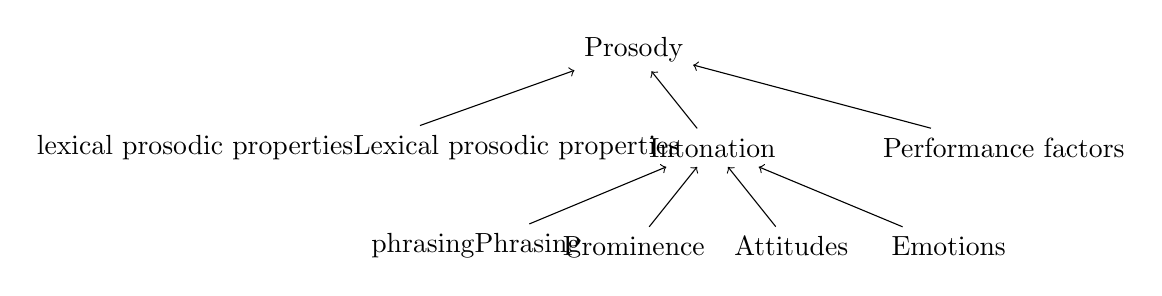
\begin{tikzpicture}
%	\node (a) at (0, 1) {\textsc{gen/num (erg)}};
	\node (b) at (1.5, 1.5) {\is{phrasing}Phrasing};
%	\node (c) at (1.5, 2.5) {\textsc{gen/num (erg)}};
%	\node (d) at (0, 2.75) {Lexically distinctive properties};
	\node (d) at (0, 2.75) {\is{lexical prosodic properties}Lexical prosodic properties};
	\node (e) at (3.5, 1.5) {Prominence};
%	\node (f) at (3, 1) {\textsc{gen/num (erg)}};
	\node (g) at (4.5, 2.75) {Intonation};
	\node (g2) at (8.2, 2.75) {Performance factors};
	\node (h) at (5.5, 1.5) {Attitudes};
	\node (i) at (7.5, 1.5) {Emotions};
%	\node (j) at (6, 1) {\textsc{gen/num (acc)}};
%	\node (k) at (9, 1) {\textsc{person (acc)}};
%	\node (l) at (9, -0.5) {Past \textit{\textbf{(Past Imperfect)}}};
%	\node (m) at (9, -1) {\textsc{person (acc)}};
	\node (n) at (3.5, 4) {Prosody};
	\foreach \from/\to in {g/h, g/i, n/d, n/g, g/b, g/e, n/g2}
	\draw [<-] (\from) -- (\to);
	\end{tikzpicture}
	\caption{A schematic representation of the components of {prosody}.}
		\label{fig:intonationREPRODUCED}
\end{figure}

The interaction between tone and intonation is then discussed in \sectref{sec:thesuperpositionoflexicaltoneandintonation}. On this basis, \sectref{sec:keyfactorsinthephoneticimplementationoftone} addresses the phonetic implementation of tone. Next, \sectref{sec:examplesofmistakeninterpretationsoftonalsequencesforwantoftakingtoneimplementationrulesintoaccount} recapitulates the various observations about tone implementation by illustrating them through examples of \is{mistakes}mistaken notations from early field notes.
Lastly, by way of conclusion, \sectref{sec:ExperimentalPhonetic} 
sets out prospects for future experimental phonetic modelling. 
%in particular the conveyance of prominence and phrasing, 
%concerning phrasing (\sectref{sec:syntacticintonationphrasingandjunctures}) and pragmatics~--  of informational prominence) (\sectref{sec:pragmaticintonation}).

\section{Syntactic intonation: Phrasing and junctures}
\label{sec:syntacticintonationphrasingandjunctures}


\is{syntactic intonation|(}

The most important unit in the prosodic organization of Na speech is the \isi{tone group}, examined in Chapter~\ref{chap:toneassignmentrulesandthedivisionoftheutteranceintotonegroups}, where much information relevant to \isi{phrasing} has already been set out in detail. From a~phonological point of view, tonal processes operate independently within each tone group. From the point of view of intonation, 
%and the phonetic implementation of tone sequences, 
however, the picture is more nuanced. On the one hand, there is a~degree of independence between tone groups; in particular, reference values of F\textsubscript{0} do not match across tone-group boundaries, as detailed in the next section. On the other hand, tone groups are integrated into higher-level prosodic units, characterized by intonational phenomena extending over several successive tone groups (\sectref{sec:higherlevelunitssentenceparagraph}).

% \subsection{Declination in fundamental frequency}
% \label{sec:resettingofreferencevaluesfortonesatjuncturesbetweentonegroups}


\subsection[Gaps in reference values at junctures between tone groups]{Gaps in reference F\textsubscript{0} values for tones at junctures between tone groups}
\label{sec:resettingofreferencevaluesfortonesatjuncturesbetweentonegroups}

Full resetting of F\textsubscript{0} does not take place at each \is{boundary (between tone groups)}boundary between two tone groups, but there can be a~sizeable \textit{discrepancy in reference values for tones} across such \is{boundary (between tone groups)}boundaries, such
that an~M tone in final position within a~\isi{tone group} and another M tone in initial position within
the following \isi{tone group} can have widely different fundamental frequency values. 

An illustration is found in the
elicited sentence (\ref{ex:horsestomach}), where the M tones of /\ipa{hu˧mi˧}/ ‘stomach’ are realized
distinctly lower than those of /\ipa{ʐwæ˧zo˧=bv̩˧}/ ‘of \mbox{(a/the)} horse’.  

\begin{exe}
	\ex
	\label{ex:horsestomach}
	\ipaex{ʈʂʰɯ˧ {\kern2pt}|{\kern2pt} ʐwæ˧zo˧=bv̩˧ {\kern2pt}|{\kern2pt} hu˧mi˧ ɲi˥.}\\ 
	\gll ʈʂʰɯ˥		ʐwæ˧zo\#˥	=bv̩˧	hu˧mi˥\$	ɲi˩\\
	\textsc{dem.prox}	colt	\textsc{poss}		stomach		\textsc{cop}\\
	\glt ‘This is the stomach
	of a~colt.’ \textit{(DetermCompounds7.140)} \pandoi{0004456\#W140}
\end{exe}

In (\ref{ex:horsestomach}),
%and (\ref{ex:idonteat}), 
the M tones in the final tone group precede an H tone, and are coarticulated accordingly: with a~lowered pitch (see \sectref{sec:tonalcoarticulationanticipatoryphoneticdissimilationinmlandmhsequences}). 

%(Monosyllabic tone groups constitute a~special case, where there are three tonal possibilities at the surface phonological level: M, LH, and MH.)

However, successive tone groups are not entirely independent from the
point of view of phonetic implementation. Rather, they are part of higher-level prosodic units characterized by intonational phenomena spanning several successive tone groups.

\subsection{Above the tone group: Sentence and prosodic paragraph}
\label{sec:higherlevelunitssentenceparagraph}
A first useful cross-linguistic descriptive concept in this space is the \textit{sentence}~-- also referred to as the \textit{utterance}, a~term that aims to bring out its grounding in a~communicative context, as emphasized by \citet{culioli1995}. No attempt will be made here to define it in any elaborate way. Let us simply note that, at sentence level, the neutral affirmative sentence is the basic,
archetypal pattern from which other sentence modes depart \citep{thorsen1980}. Abstracting away from other dimensions of \isi{prosody} (such as \isi{lexical prosodic properties}, prominence, and the expression of attitudes and emotions), the
F\textsubscript{0} curve of a~sentence typically rises to a~peak located on one of its first syllables. The gradual, noncategorical decrease in fundamental frequency known as \is{declination|textbf}‘{declination}’ takes place over the course of the sentence. Fundamental frequency thus fluctuates within a~gradually narrowing
range, until {final lowering}, which signals the end of the sentence. (This corresponds to Tune 1 as described for
\ili{English} by \citealt{armstrongetal1926}.) 


\is{final lowering|textbf}Final lowering is a~more localized phenomenon, typically
affecting the last syllable of declarative utterances, but this is subject to cross-language \isi{variation}.

\begin{quotation}
	Final lowering can be total, leading to the neutralisation of High and Low tones, as in \ili{Akan}. It can be realized as a~low register plateau, as in \il{Chichewa}Chi\-che\-wa or in \ili{Bemba} (for the long stretched one), or as a~gradual fall, as in \ili{Embosi}, or as a~sharp fall, as in \ili{Bemba} (for the one syllable one). Its domain can be short (one syllable) or rather long (a stretch of tone bearing units). \citep[4-5]{downingrialland2016}
\end{quotation}

Declination and final lowering are common across languages, as is their suspension to convey
non-assertiveness (in questions, or to convey nuances of doubt and uncertainty). 

Studies of read speech in languages such as \ili{English} or \ili{French} note that the peak F\textsubscript{0} value in a~sentence tends to decrease from the
first to the last sentence in a~paragraph \citep{lehiste1975}. Paragraph-final position is typically characterized by an~extra-low F\textsubscript{0}, often accompanied by a~change in phonation type and reduced intensity \citep[50–52]{vaissiereetal2006}. 
On the analogy of written text, it has been proposed to refer to \textit{prosodic paragraphs} as a~unit above sentence level in spontaneous speech \citep{grobet2001differents}. The term ‘paragraph’ has been criticized by linguists who object to applying concepts from written text analysis to spoken language. Nevertheless, it remains a~convenient label, in view of the similarities between the division of a~written text into paragraphs and that of speech into prosodic paragraphs~-- both of which allow for a~high degree of \is{stylistics}stylistic freedom. 

%In Yongning Na, \isi{declination} is most transparently observed in sentences that have long sequences of like tones: M..M or L..L.\footnote{Remember that H..H sequences are ruled out by the fact that H tone is culminative: there can be at most one H~tone in a~\isi{tone group}. All tones following H are depressed to L: see \sectref{sec:alistoftonerules}.}

From a~phonetic point of view, prosodic phenomena at the levels of the sentence and the prosodic paragraph interact with tones. The phonetic
realization of a~phonological H, M or L differs considerably depending on the position of the
syllable within the sentence and the prosodic paragraph. For instance, in Yongning Na, the 1\textsuperscript{st}, 2\textsuperscript{nd}, and 3\textsuperscript{rd}-person pronouns //\ipa{njɤ˩}//, //\ipa{no˩}//, and //\ipa{ʈʂʰɯ˥}// all have M tone \is{form!in isolation}in isolation due to the \isi{neutralization}~-- in this position~-- of the lexical categories L, M, and H. Their surface phonological representation \is{form!in isolation}in isolation is therefore /\ipa{njɤ˧}/, /\ipa{no˧}/, and
/\ipa{ʈʂʰɯ˧}/, respectively. But in my first notes I transcribed them with H tone, as [\ipa{njɤ˥}],
[\ipa{no˥}], and [\ipa{ʈʂʰɯ˥}]. This was due to their realization on a~high pitch \is{form!in isolation}in isolation. In that
context, their pitch is noticeably higher than that of an~M tone occurring in tone-group-initial position later
within a~prosodic paragraph.

Thus, in my first field notes, I transcribed (\ref{ex:idonteat}) as $\ddagger${\kern2pt}\ipa{njɤ˥ mɤ˧-dzɯ˥}; I was led to
this phonologically inappropriate notation by the considerable phonetic difference in pitch between the first and second syllables, as well as the similarity in pitch between the first and last syllables of this short
sentence. The effects of phrasing and coarticulation had to be brought to light before a~correct transcription of the
surface phonological form of the pronouns could be arrived at. 

\begin{exe}
	\ex
	\label{ex:idonteat}
	\ipaex{njɤ˧ {\kern2pt}|{\kern2pt} mɤ˧-dzɯ˥.}\\ 
	\gll njɤ˩	mɤ˧-	dzɯ˥\\
	\textsc{1sg}		\textsc{neg}		to\_eat\\
	\glt ‘I don’t eat.’
\end{exe}

% see, among other examples, the contrast between the phonetic realization of
%/\ipa{njɤ˧}/ ‘I’ and /\ipa{ə˧si˧}/ ‘grandmother’ in /\ipa{njɤ˧} {\kern2pt}|{\kern2pt}
%\ipa{ə˧si˧}/ ‘my grandmother’ in Dog.56. 

\is{syntactic intonation|)}

\section{Pragmatic intonation}
\label{sec:pragmaticintonation}

“Information structure is a~vast topic of research that has been pursued within different theoretical frameworks” \citep[244]{krifka2008}, and with different objectives in view. A~few general observations about \isi{information structure} in Yongning Na will be followed by a~discussion of two phenomena that belong to \textit{pragmatic intonation}: \isi{emphatic stress} (\sectref{sec:emphaticstressanditstoneddownavatars}) and \isi{focalization} through local intonational modification of tone (\sectref{sec:focalization}).\footnote{This section contains passages adapted from \citet{michaudetal2016}.}
%, and (iii)~intonational backgrounding of \isi{function words} (\sectref{sec:intonationalbackgroundingofparticles}).

The following observations about Qiang (\ili{Rma}) also apply to Yongning Na (and other \il{Sino-Tibetan}Sino-Tibetan languages): 

\begin{quotation}
	 \begin{sloppypar} % To avoid overfull hbox. For 2nd edition: tried to be brave & try to do without sloppy paragraphs. Did not work.
	The structure of the clause is to some extent affected by pragmatic factors, but this only applies to the order of noun phrases in the clause. The utterance-initial position is the unmarked topic position (though secondary topics can follow the primary topic), while the position immediately before the verb is the unmarked focus position, and so the focused element will generally appear there. The verb always appears in final position; there is no possibility for the actor of a~clause to appear in postverbal position, even if it is focal. The only \is{exceptions}exception to this is the occasional afterthought clarification of a~noun phrase that was omitted or expressed as a~\is{pronouns}pronoun in the clause. \citep[221]{lapollaetal2003a}
	\end{sloppypar}
\end{quotation}

%Command \noindent added to avoid having an indent. Proofreader suggestion: since this sentence continues the argument, it is better not to indent. 
{\noindent}Information structure in Na has accordingly been described as ‘topic-comment’, extending an observation made by Chao Yuen-ren about \ili{Sinitic}: “the grammatical meaning of subject and predicate in a~\il{Sinitic}Chinese sentence is topic and comment, rather than actor and action” (\citealt[69]{chao1968}; see also \citealt{shi2000}; \citealt{lapolla2009}). 
\begin{quotation}
The primary \isi{information structure} in Na is topic/comment rather than subject/predicate. ({\dots}) [A]~topic can be a~nominal argument, which the rest of the sentence will comment upon, but the topic can also be an {adverbial}, an independent clause, or a~dependent clause. \citep[296]{lidz2010}
\end{quotation}

Example (\ref{ex:stomachache}) provides an illustration. 

\begin{exe}
	\ex
	\label{ex:stomachache}
	\ipaex{le˧-dzɯ˥ {\kern2pt}|{\kern2pt} bi˧mi˧ go˩.}\\ 
\gll le˧-			dzɯ˥		bi˧mi˧			go˩\textsubscript{a}\\
\textsc{accomp}		to\_eat 		stomach/belly 		to\_ache\\
  \glt ‘[If] [you] eat [of it], [your] stomach [will] hurt!’ (Field notes. Context: on the mountain, pointing out a~berry that is not edible.)
\end{exe}


\subsection{Emphatic stress and its toned-down avatars}
\label{sec:emphaticstressanditstoneddownavatars}

\is{emphatic stress|textbf}

An ‘up’ arrow \ipa{↑} placed to the left of a syllable indicates \isi{emphatic stress}, as in (\ref{ex:theelderwasaboy}).

\begin{exe}
  \ex
  \label{ex:theelderwasaboy}
  \ipaex{tʰi˩˥, {\kern2pt}|{\kern2pt} ə˧mv̩˧ ʝi˥-hĩ˩ {\kern2pt}|{\kern2pt} -dʑo˩, {\kern2pt}|{\kern2pt} ↑zo˧ ɲi˥ tsɯ˩ {\kern2pt}◊{\kern2pt} mv̩˩.}\\
  \gll tʰi˩˥		ə˧mv̩˧˥		ʝi˥ 	-hĩ˥		dʑo˥ zo˥ 		ɲi˩ 	tsɯ˧˥	mv̩˧\\
  then 	elder\_sibling	to\_do	\textsc{rel}	\textsc{top} boy/son 	\textsc{cop}
  \textsc{rep}	\textsc{affirm}\\
  \glt ‘The elder [of the two siblings] was a~boy.’ \textit{(Sister.5)} \pandoi{0004341\#S5}
\end{exe}

In many contexts, \isi{emphatic stress} appears on a~constituent that can be predicted to receive focus \isi{prosody}. For example, in sentence (\ref{ex:theelderwasaboy}), one would expect the focus to be in the immediate preverbal position~-- the usual unmarked focus position in verb-final languages. Emphatic stress can thus be viewed as an extreme form of focus \isi{prosody}~-- an extreme along a~continuum: there is no hard-and-fast {boundary} between \isi{emphatic stress} and milder realizations of focus \isi{prosody}. 

Emphatic stress %is phonetically located on a~single syllable, but from the point of view of interpretation,
presents an interpretative ambiguity: it may signal either {\linebreak}“broad focus” or “narrow focus”, to use terms proposed by \citet{lambrecht1994}. This phenomenon is extensively studied in the literature on focus projection (e.g.~\citealt{selkirk1995}). 

The phonetic realization of \isi{emphatic stress} includes effects on the articulation of vowels and consonants. For instance, in (\ref{ex:playingwith}), the second syllable of /\ipa{dʑɤ˩↑bv̩˥}/ ‘to play’ is realized with stronger trilling of the /\ipa{b}/ than is found in non-emphatic contexts. 
This can be considered an example of ‘articulatory prosodies’ in the sense of \citet{kohleretal2011} and \citet{niebuhr2013}.

\begin{exe}
	\ex
	\label{ex:playingwith}
	\ipaex{mv̩˩zo˩=ɻæ˩ lɑ˥ {\kern2pt}|{\kern2pt} ə˧ʝi˧-ʂɯ˥ʝi˩ {\kern2pt}|{\kern2pt} tʰi˩˥, {\kern2pt}|{\kern2pt} dʑɤ˩↑bv̩˥-ɲi˩ tsɯ˩ {\kern2pt}◊{\kern2pt} mv̩˩!}\\
	\gll mv̩˩zo˩		=ɻæ˩		lɑ˧ 	ə˧ʝi˧-ʂɯ˥ʝi˩		tʰi˩˥		dʑɤ˩bv̩˥ 		-ɲi˩ 	tsɯ˧˥	mv̩˧\\
	girl	\textsc{associative}	with	long\_ago	so/then	to\_play		\textsc{certitude}
	\textsc{rep}	\textsc{affirm}\\
	\glt ‘The story goes that at that time, long ago, he would have fun [i.e.\ flirt] with girls!’ \textit{(Caravans.231)} \pandoi{0004530\#S231}
\end{exe}

%\subsubsection{Emphatic stress as a~language universal}
\label{sec:emphaticstressasalanguageuniversal}

Emphatic stress in Na appears to be essentially the same phenomenon as in \ili{English} and \ili{French}, motivating the adoption of this label (proposed by \citealt{coustenobleetal1937}). Prototypical realizations of emphatic
stress have been shown to involve supplementary activity of the expiratory muscles, resulting in
a~sudden rise in subglottal pressure during the articulation of a~consonant
\citep{benguerel1973,cartonetal1976,ohala1978,fantetal1996}, hence the term “force-accent” used by \citet{kohler2003}. 

This category has been somewhat neglected in \isi{intonation} studies, as the dominance of tonal models
of \isi{intonation} led researchers to focus their attention mostly on the acoustic parameter of
fundamental frequency. But it is a~good candidate for the status of universal of human language. It is the most
extreme manifestation of intonational emphasis, with
linguistic functions ranging from attitudinal and emotional to pragmatic. 

In speech, toned-down realizations of \isi{emphatic stress} are more common than its prototypical realization: the physiological effort at the~subglottal level is often mimicked through such strategies as
F\textsubscript{0} excursions and consonant \isi{lengthening}. Needless to say, the
description of \isi{emphatic stress} as a~language universal by no means implies that it is uniformly present in all
languages and all oral genres. Like other linguistic phenomena, it comprises important
language-specific and speech-style-specific dimensions. Its frequency of use varies greatly from
language to language, from speaker to speaker, and from style to style; its \is{stylistics}stylistic effect is
inversely proportional to its frequency of use.


\subsection[Focalization by intonational means]{Focalization through local intonational modification of tone}
\label{sec:focalization}

\is{focalization|textbf}

%\subsubsection*{The main facts}
\label{sec:themainfactsfocalization}

In Yongning Na, there can be \isi{focalization} through local intonational modification of tone on the last syllable of the word in focus. The syllable gets \is{lengthening}lengthened. An~H or M level tone changes to a~dipping {contour}, while the phonetic range of an~MH or LH rising {contour} gets expanded. As for L tone, which is canonically realized with a~decrease in fundamental frequency, its falling {contour} becomes more noticeable under \isi{focalization}. This phenomenon will be referred to, for short, as \textit{intonational focalization}. 

The notation
adopted is ‘\ipa{F}’ (for ‘Focalization’), placed after the syllable at issue. This may seem inconsistent
with the choice to place the upward arrow for \isi{emphatic stress} (\ipa{↑}) \textit{before} the stressed syllable (\sectref{sec:emphaticstressanditstoneddownavatars}). There is a~phonetic basis for this different treatment, however: while \isi{emphatic stress} is strongest at the \textit{onset} of
the syllable, intonational \isi{focalization} primarily affects the syllable \textit{rhyme}.

This phenomenon was first identified in examples where the syllable receiving this intonational modification carried H~tone. The modification of H~tone is more conspicuous than that of M, L, MH or LH: its realization becomes a~rapid dipping
{contour}, for instance in examples (\ref{ex:shedidnotgreetanyone}) and (\ref{ex:nogift}).

\begin{exe}
  \ex
  \label{ex:shedidnotgreetanyone}
  \ipaex{hĩ˧-ki˧ {\kern2pt}|{\kern2pt} ɖɯ˧-kʰwɤ˥ F {\kern2pt}|{\kern2pt} mɤ˧-pi˥!}\\
  \gll hĩ˥		-ki˧	ɖɯ˧-kʰwɤ˥\$		mɤ˧-	pi˥\\
  person	\textsc{dat}	1-\textsc{clf}.pieces	\textsc{neg}	to\_say\\
  \glt ‘(S)he did not say anything to the people present! / (S)he did not greet anyone!’ (Field
  notes, 2009)
\end{exe}

\begin{exe}
	\ex
	\label{ex:nogift}
	\ipaex{no˧ {\kern2pt}|{\kern2pt} njɤ˧-ki˧ {\kern2pt}|{\kern2pt} ɖɯ˧-sɑ˥ F {\kern2pt}|{\kern2pt} hwæ˧-mɤ˧-zo˧!}\\
	\gll no˩	njɤ˩		-ki˧		ɖɯ˧-sɑ˥\$				hwæ˧\textsubscript{a}		mɤ˧-		-zo˧\textsubscript{a}\\
	\textsc{2sg}	\textsc{1st}	\textsc{dat}	1-\textsc{clf}.things		to\_buy		\textsc{neg}		\textsc{oblig}\\
	\glt ‘You don't need to give me anything! / There is no need to buy any presents for me!’ \textit{(TraderAndHisSon.34)} \pandoi{0004632\#S34}
\end{exe}

In (\ref{ex:shedidnotgreetanyone}), the \is{numerals}numeral-plus-classifier phrase /\ipa{ɖɯ˧-kʰwɤ˥}/ ‘one piece’ is given {\linebreak}\isi{prominence} through the phonetic realization of the classifier /\ipa{kʰwɤ˥}/ with a~noticeable fall plus \isi{lengthening}. Likewise for /\ipa{ɖɯ˧-sɑ˥}/ ‘anything’ (literally ‘one thing’) in (\ref{ex:nogift}). A~spectrogram illustrating this phenomenon is shown in \figref{fig:noneedforbuying}.

\begin{figure}[ht]
	\includegraphics[width=\textwidth]{figures/F/F.pdf}
	\caption{Spectrogram and F\textsubscript{0} curve for example (\ref{ex:nogift}), showing a~noticeable fall plus {lengthening} on the syllable /\ipa{sɑ˥}/ in /\ipa{ɖɯ˧-sɑ˥}/ ‘anything’. Top line of annotation: segments; bottom line: tones, with the added mention ‘+Foc’ for the syllable receiving intonational {focalization}.}
	\label{fig:noneedforbuying}
\end{figure}

This phenomenon is found in rapid speech as well as in slow repetitions.

It was later realized that the same type of \isi{prominence}-lending local intonational modification also applied to the two rising contours: high-rising (MH) and low-rising (LH). For these
contours, the effect consists of \isi{lengthening} and F\textsubscript{0} \isi{range expansion}. Since these are already phonological contours, which have inherently greater \isi{duration} than simple levels, the modification is less salient perceptually than for M
and H. Recognition of the existence of this phenomenon for the L level came last.

On the {analogy} of \ili{Naxi}, where a~reduced M- or L-tone syllable can give rise to contours \citep{michaudetal2007d} that bear some phonetic similarity to those of Yongning Na, it was first hypothesized that a~reduced
syllable must be present in examples such as (\ref{ex:shedidnotgreetanyone}): $\ddagger${\kern2pt}\ipa{ɖɯ˧-kʰwɤ˥-ə˩
  mɤ˧-pi˥}. Likewise, example (\ref{ex:invitationtoeat}) was initially transcribed as $\ddagger${\kern2pt}\ipa{ə˧-dzɤ˧${\sim}$dzɤ˥-ə˩
  dzɯ˧}. Subsequent investigation showed that these notations were inappropriate, however. The observed dip in
fundamental frequency, accompanied by \isi{lengthening}, is
a~purely intonational device, not an indication of an additional syllable.

%\Hack{\newpage}

\begin{exe}
	\ex
	\label{ex:invitationtoeat}
	\ipaex{ə˧-dzɤ˧${\sim}$dzɤ˥ F {\kern2pt}|{\kern2pt} dzɯ˧!}\\ 
	\gll ə˧-dzɤ˧${\sim}$dzɤ˥		F			 	dzɯ˥\\
	slowly		\textsc{focalization}		to\_eat\\
	\glt ‘Eat slowly!/Take your time!’ (Polite invitation to eat.)
\end{exe}

The realization of \isi{focalization} comprises a~movement in F\textsubscript{0}, a~slight \isi{lengthening}, and perhaps a~slight change in the vowel, as if a~final \textit{schwa} target were added. This process is specific enough for tonal distinctions to be preserved: headlong conflict with the underlying tone system is avoided. To put it differently, intonational \isi{focalization} does not lead to \isi{neutralization} of lexical tone. Similarly, emphatic stress remains perceptually distinct from lexical tone, as it is cued by various phonetic dimensions beyond fundamental frequency. The possibility of a~\isi{misperception} of lexical tone caused by intonational phenomena is therefore limited.


\largerpage[2]
\subsection{Borderline cases}
\label{sec:borderlinecasesopeningintoadiscussionofthecategoricalstatusofthephenomenon}


About two hundred instances of intonational \isi{focalization} are indicated in the first twenty transcribed
texts. Some cases are clearer than others. For one thing, cases where this \isi{focalization} is
superimposed on rising contours, and on L tones, tend to be less salient perceptually for phonetic reasons, as mentioned above. For another, there are borderline cases, where it is not obvious whether to add a~‘\ipa{F}’ in the
transcription or not. Borderline cases do not by themselves cast doubt on the categorical nature of the phenomenon. Intonational \isi{focalization} can be toned down, in the same way as \isi{emphatic stress} has toned-down avatars shading into non-emphatic realizations; this is a~common situation in the field of \isi{intonation}. On the other hand, it should be borne in mind, when consulting the texts, that the ‘\ipa{F}' and ‘\ipa{↑}' symbols (for intonational \isi{focalization} and \isi{emphatic stress}, respectively) cannot be assigned with the same degree of certainty as consonants, vowels, and tones. For instance, the syllable /\ipa{li˩}/ ‘to see’ is transcribed in (\ref{ex:FLex})\footnote{In (\ref{ex:FLex}), the second and third syllables of /\ipa{ʈʂʰɯ˧ne˧-ʝi˥}/ ‘thus’ are coalescent, and fully undistinguishable on the spectrogram (\figref{fig:FL}). For convenience, a~simplified transcription as [\ipa{ʈʂʰɯ˧ne˧ gv̩˧˥}] is adopted in the surface phonological transcription of the sentence, and in the annotation to the spectrogram, in preference to /\ipa{ʈʂʰɯ˧ne˧-ʝi˧ gv̩˧˥}/. This case of coalescence is analyzed in Appendix A, \sectref{sec:smoothphoneticonsets}.} with an indication of intonational \isi{focalization}, on the basis of the auditory impression that it stands out in the flow of speech. The proposed translation for /\ipa{hĩ˧ li˩ F mɤ˩-ʁo˩}/ in (\ref{ex:FLex}) is ‘{\dots}~could not \textit{even} see people’, chosen to reflect the pragmatic implications of focalization on the verb ‘to see’. The sequence /\ipa{hĩ˧ li˩ mɤ˩-ʁo˩}/, without intonational \isi{focalization}, would simply mean ‘{\dots}~could not see people’. 

\begin{exe}
	\ex
	\label{ex:FLex}
	\ipaex{le˧-mo˩, {\kern2pt}|{\kern2pt} le˧-mo˩, {\kern2pt}|{\kern2pt} njɤ˩ɭɯ˧ {\kern2pt}|{\kern2pt} ʈʂʰɯ˧ne˧ gv̩˧˥, {\kern2pt}|{\kern2pt} hĩ˧ li˩ F mɤ˩-ʁo˩!}\\ 
	\gll le˧-				mo˩\textsubscript{a}		njɤ˩ɭɯ˧		ʈʂʰɯ˧ne˧-ʝi˥		gv̩˧\textsubscript{c}				hĩ˥		 li˧\textsubscript{a}	F	mɤ˧-		ʁo˧\\
	\textsc{accomp}		old								eye				thus				to\_occur		person		to\_look\_at	\textsc{focalization}	\textsc{neg}		to\_be\_able\_to/to\_manage\\
	\glt ‘[The dog] got older and older; and so, its eyes could not even look at people anymore / it could not even see people anymore!’ \textit{(Dog2.80)} \pandoi{0004555\#S80}
\end{exe}

But looking at the spectrogram in \figref{fig:FL}, it appears that the syllable /\ipa{li˩}/ ‘to see’ is not strikingly different from its neighbours in terms of either \isi{duration} or fundamental frequency. The average fundamental frequency of vowel /\ipa{i}/ in /\ipa{li˩}/ is two semitones lower than that of /\ipa{ĩ}/ in the preceding syllable, /\ipa{hĩ˧}/ (210~Hz vs.\ 237~Hz), a~phonetic difference that is in keeping with the phonological tones (M vs.\ L). The decrease in fundamental frequency between /\ipa{li˩}/ and the two L-tone syllables that follow can be interpreted as a~straightforward case of \is{declination}\textit{declination}, a~phenomenon mentioned in \sectref{sec:syntacticintonationphrasingandjunctures}.  


\begin{figure}[b]
	\includegraphics[width=1.03\textwidth]{figures/FL/FL.pdf}
	\caption{Spectrogram and F\textsubscript{0} curve for example (\ref{ex:FLex}), showing a~slight fall plus hints of {lengthening} on the syllable /\ipa{li˩}/ ‘to see’. Top line of annotation: segments; bottom line: tones, with the added mention ‘+Foc’ for the syllable presumed to receive intonational focalization.}
	\label{fig:FL}
\end{figure}
The data is nonetheless compatible with the hypothesis (based on auditory impression) that the syllable /\ipa{li˩}/ ‘to see’ is highlighted by intonational means. In terms of \isi{duration}, the syllable /\ipa{li˩}/ is 20~centiseconds long, which is slightly above the average for the passage shown in \figref{fig:FL} (100 centiseconds for seven syllables, i.e.\ about one syllable every 15 centiseconds). This difference in length cannot be dismissed as linked to the syllable's phonemes: if anything, the vowel /\ipa{i}/ would be expected to be intrinsically \textit{shorter} than other vowels \citep{dicristoetal1986, whalenetal1998}. As for fundamental frequency, the display in \figref{fig:FL}, covering the range from 0~Hz to 450~Hz, gives the impression of a~relatively smooth curve over the last four syllables, but if the scale is changed to a~narrower range, as in \figref{fig:FLCloseup}, the hump at the beginning of the vowel /\ipa{i}/ in /\ipa{li˩}/ becomes more salient visually. This hump, which results in a~dip of 2.5 semitones in the brief course of this vowel, could be significant: there is no obvious contextual reason why the hump should be present, therefore it makes sense to interpret it as one of the phonetic correlates of a~local intonational modification signalling some sort of emphasis, such as the phenomenon of intonational \isi{focalization} transcribed here as ‘\ipa{F}’.


\begin{figure}[ht]
	\includegraphics[width=1.03\textwidth]{figures/FL/FLCloseup.pdf}
	\caption{Same data as in \figref{fig:FL}, adopting a~narrower range for F\textsubscript{0} display.}
	\label{fig:FLCloseup}
\end{figure}

When transcribing narratives, one way to check with the speaker whether to classify a~given case as having intonational \isi{focalization} or not consists in playing the passage at issue, then repeating it with and without the telltale fall in pitch and \is{lengthening}lengthened rhyme, and asking the consultant to indicate which of the two realizations fits better. But this entails no guarantee: even supposing that the investigator is successful in producing the intended distinction, the consultant may not base her decision on the realization heard on the recording. She may go for the realization which she considers (in retrospect) would have been more suitable in that context. 


Pending experimental verification through perceptual tests, it seems likely that different speakers have different degrees of sensitivity to intonational detail. Toned-down versions of intonational \isi{focalization} may go unnoticed by some speakers. It is a~fact of life that hearers can fail to pick up intended clues. A~linguist's aphorism has it that, in human communication, misunderstanding is the general case, and mutual understanding is a~special case (``la compréhension est un cas parti\-culier du malentendu'': \citealt[39]{culioli1990}).
The world is a~cemetery of cultures, and every text a~tomb for lost allusions.\footnote{Lost allusions are often staged in literary works, among them Proust's \textit{In Search of Lost Time}. The grandmother's sisters design allusions that are so carefully veiled that they are unintelligible to the intended addressees: ``{\dots}~they, in their horror of vulgarity, had brought to such a~fine art the concealment of a~personal allusion in a~wealth of ingenious circumlocution, that it would often pass unnoticed even by the person to whom it was addressed.'' Scott Moncrieff translation revised by Terence Kilmartin. \textit{Original text:} <<~Celles-ci par horreur de la vulgarité poussaient si loin l’art de dissimuler sous des périphrases ingénieuses une allusion personnelle qu’elle passait souvent inaperçue de celui même à qui elle s’adressait.~>>} 



\section{Tone and intonation: Superposition and interaction}
\label{sec:thesuperpositionoflexicaltoneandintonation}

The observations presented separately about two major components of \isi{intonation}~-- \isi{phrasing} in \sectref{sec:syntacticintonationphrasingandjunctures} and \isi{prominence} in \sectref{sec:pragmaticintonation}~-- now call for an account of how they combine with each other, as well as with tone. It is all very well to distinguish different functional levels: in
particular, tone on the one hand, and intonational modifications on the other. But since tone and \isi{intonation} share a~key phonetic parameter~-- fundamental frequency~--, a~phonetic issue is bound to arise: how is information from the different functional levels conveyed through the same acoustic channel? 

The general approach adopted here is \is{superpositional (approaches to prosody)}superpositional, in keeping with Chao Yuen-ren's intuition of tones as ripples riding over a~larger wave (sentence intonation). The various components are conceived as superimposed: local modulations (reflecting tones, intonational focalization and emphatic stress, as well as phrasing) are grafted onto an overall sentence-level pattern that depends on sentence mode and speaker attitude (and emotion)~-- with some phenomena operating over wider domains such as the \textit{prosodic paragraph}. Thus, the analytical baseline consists in assuming that the functional distinction between lexical tones and \isi{intonation} is preserved: that listeners process F\textsubscript{0} curves in such a~way as to retrieve both tone and intonation, teasing them apart in perception, as it were. 


Against this general background, a~range of different situations are observed in practice. A compromise has to be found, in each speech act, between the competing demands of clarity, on the
one hand, and \is{expressivity}expressivity, on the other. Depending on context, the relative weight of these two components can be very different. For instance, when picking up the phone, speakers of \ili{Mandarin} say \textit{wèi} \zh{喂}, lexically a~tone-4 syllable, i.e.\ with sharply falling pitch; but in this context,
the lexical tone can be overridden by interrogative \isi{intonation}, and the pitch is often rising. One theoretically possible interpretation would be that the lexical tone, tone 4, is changed to another, say, tone 2, the rising
tone. But rather than treating this case as an~instance of tone change, it makes better sense to
consider it as an extreme case where the lexical tone has so little communicational relevance,
and the expression of speaker attitude such importance, that the end result bears little trace (if any) of the lexical tone.

As a~general rule, it seems clear that Na speakers are careful to avoid too
great a~distortion of the tonal string due to intonational emphasis. While no specific phonetic
study has so far been conducted on Yongning Na data, it seems reasonable to assume that the
situation is comparable to \ili{Naxi}, where a~study of the three basic tones (H, M and L) under emphasis reveals a~proportionally milder effect of emphasis on F\textsubscript{0} than on
intensity, as compared to \ili{English} data (\citealt[107–167]{michaud2005}; \citealt{michaudetal2015d}). 

There are nonetheless cases in which pragmatic intonation interacts with tones to the point of tampering with the tonal string. Such cases are analyzed below. Rather than dismissing them as marginal, it seems more forward-looking to heed the suggestion of \citet{marsault2024_ideophones} and \citet[258]{dingemanse_interjections_2024} to pay special attention to elements traditionally considered as peripheral~-- an approach that is seemingly iconoclastic but turns out to be highly heuristic.

\subsection{Influence of emphatic stress on the tonal string}
\label{sec:caseswhereintonationinteractswiththetonalstring}

In some rare cases, intonational modifications go so far as to affect the string of tones for
the utterance. In its most vehement manifestations, \isi{emphatic stress} intrudes into
a~sentence’s \isi{prosody}, wreaking havoc on tonal contrasts. Example (\ref{ex:canbecomereallywhite}) is
a~case in point.

\begin{exe}
  \ex
  \label{ex:canbecomereallywhite}
  \ipaex{pʰv̩˩-tɕæ˥ɻæ˩ gv̩˩-kv̩˩-ze˩ {\kern2pt}◊{\kern2pt} mæ˩!}\\
  \gll pʰv̩˩-tɕæ˩ɻæ˥	gv̩˧	-kv̩˧˥		-ze˧\textsubscript{b}		mæ˧\\
  very\_white	to\_become	\textsc{abilitive}	\textsc{pfv}	\textsc{affirm}\\
  \glt ‘[after boiling, linen thread] can become really white!’ \textit{(FoodShortage.73)} \pandoi{0004557\#S73}
\end{exe}

The usual pronunciation is /\ipa{pʰv̩˩-tɕæ˩ɻæ˥}/ ‘very white’. In (\ref{ex:canbecomereallywhite}),
the second syllable is realized phonetically with extremely high fundamental frequency on the
syllable /\ipa{tɕæ˩}/, which is also considerably \is{lengthening}lengthened. From a~phonetic point of view, its phonetic
L tone is conspicuously disregarded. One way of looking at this modification would be to describe it
as due to an~intonational overlay: functionally, one could consider transcribing as
/\ipa{pʰv̩˩-↑tɕæ˩ɻæ˥-gv̩˩}/, where the arrow \ipa{↑} indicates \isi{emphatic stress}, and the phonological
tonal string is unchanged.

This forcible intonational modification does interact with the phonological tone string of the tone
group, however. If the modification of the second syllable in /\ipa{pʰv̩˩-tɕæ˩ɻæ˥-gv̩˩}/ only took
place on an~intonational level, one would expect the phonological tonal string to remain unchanged, in
which case the third syllable would retain its phonological H tone. But what is observed is that the
third and fourth syllables in (\ref{ex:canbecomereallywhite}) are lowered to L:
/\ipa{ɻæ˩-gv̩˩}/. This is precisely what is expected if the second syllable carries H tone. This
phenomenon is therefore analyzed as involving a~categorical tone change, from an~L.L.H sequence, /\ipa{pʰv̩˩-tɕæ˩ɻæ˥}/, to an~L.H.L sequence, /\ipa{pʰv̩˩-tɕæ˥ɻæ˩}/.

This example illustrates how an \is{expressivity}expressive coinage possessing 
%and \is{iconicity}iconic phenomena constitute marginal elements: each of them has 
a~lilt of its own undergoes continuous attraction from the more central structures that make up the language's phonological system, tending towards its integration into the language's phonological categories, and interacting with these categories in the process. 
%~-- an integration which has potential for causing modifications to the system. 

%(Segmental examples of this phenomenon are discussed in Appendix A, \sectref{sec:expressivecoinagesandmore}.) As the association of emphatic stress to a~given item becomes more frequent, the way towards lexicalization is gradually paved. 

Another example where emphatic stress interacts with tone~-- in this case obscuring a~syllable's lexical tone~-- consists of the set of eight extra-distal locative expressions, which share a~specific \isi{intonation}. The argument proposed here is that this habitual intonation constitutes a~path towards the loss of lexical tone on the grammatical morphemes at issue. These locative expressions are listed in \tabref{tab:expressivelocatives}, where their first syllable is transcribed with an exclamation mark ‘!’ instead of a~tone mark, as a~provisional device to represent their telltale \isi{intonation}. 

\begin{table}%[t]
	\caption{Extra-distal locative expressions carrying specific {intonation}.}
	\begin{tabularx}{\textwidth}{ l Q l@{\hspace{10mm}} l }
		\lsptoprule
		locative & meaning & 1\textsuperscript{st} σ & meaning of 1\textsuperscript{st} σ\\\midrule
		\ipa{gɤ!-qo˧} & way up & \ipa{gɤ˩-} & upward\\
		\ipa{gɤ!-ʈʂʰɯ˧qo˧} & way up there (\textsc{prox}) & \ipa{gɤ˩-} & upward\\
		\ipa{gɤ!-tʰv̩˧qo˧} & way up there (\textsc{dist}) & \ipa{gɤ˩-} & upward\\
		\ipa{gɤ!-tʰv̩˧-gi\#˥} & way up in that direction & \ipa{gɤ˩-} & upward\\ \addlinespace \hdashline \addlinespace
		\ipa{dɤ!-qo˧} & way over there & ? & ?\\
		\ipa{dɤ!-ʈʂʰɯ˧qo˧} & way over there (\textsc{prox}) & ? & ?\\
		\ipa{dɤ!-tʰv̩˧qo˧} & way over there (\textsc{dist}) & ? & ?\\
		\ipa{dɤ!-tʰv̩˧-gi\#˥} & way over in that direction & ? & ?\\
		\lspbottomrule
	\end{tabularx}
	\label{tab:expressivelocatives}
\end{table}

The two sets of extra-distal locatives presented in \tabref{tab:expressivelocatives} are structurally parallel, and they share the same \isi{intonation}. The realization of their first syllable is highly \is{expressivity}expressive and allows
variants. Either it starts on an~extra-high pitch and glides downward, at a~slope left to the
speaker’s discretion: a~sharp fall or a~prolonged descent. Or it is rising, the details of the rise
(\isi{duration}, slope, and peak height) being again left to the speaker’s discretion. As far as could be
ascertained, the sharply falling \is{variants}variant emphasizes the great distance to the place at issue
(paraphrase: ‘in a~place far, far away’), whereas the rising \is{variants}variant (exemplified in \figref{fig:distalrising}) is used to direct the listener’s
attention to that place, against a~background of shared knowledge (paraphrase: ‘that faraway
place, you know’). Consider  (\ref{ex:yourdaughteriswayoverthere}), for instance: the context to this example is that a~mother thinks that her daughter has died; the young woman's lover tells the mother that her daughter is still alive, and that she is in hiding. The young man knows where the young woman is, but does not wish to disclose it to the mother. The extra-distal locative in (\ref{ex:yourdaughteriswayoverthere}) does not emphasize the great distance: paraphrase as ‘Your daughter is in a~faraway place’ would be inappropriate. In this context, the syllable /\ipa{dɤ}/ in \ipa{dɤ!-tʰv̩˧qo˧}/ ‘way over there’ is realized as rising: see the fundamental frequency tracing in \figref{fig:distalrising}.

\begin{exe}
	\ex
	\label{ex:yourdaughteriswayoverthere}
	\ipaex{no˧ mv̩˩  {\kern2pt}|{\kern2pt} dɤ!-tʰv̩˧qo˧ dʑo˩.}\\ 
	\gll no˩	mv̩˩˥		dɤ!-tʰv̩˧qo˧	dʑo˩\textsubscript{b}\\
	\textsc{2sg}	daughter	\textsc{dem.extra\_distal}		\textsc{exist}.animated\_beings\\
	\glt ‘Your daughter is [in a~place that I know,] way over there.’ {\newline}\textit{(BuriedAlive3.105)} \pandoi{0004538\#S105}
\end{exe}

\begin{figure}[ht]
	\includegraphics[width=\textwidth]{figures/Xdistal/distal.pdf}
	\caption{Spectrogram and F\textsubscript{0} curve for example (\ref{ex:yourdaughteriswayoverthere}), showing the rising realization of the syllable /\ipa{dɤ}/ in /\ipa{dɤ!-tʰv̩˧qo˧}/ ‘way over there’.}
	\label{fig:distalrising}
\end{figure}

The perceived pitch of the syllable /\ipa{dɤ}/ in these locative expressions could be stylized by means of Chao Yuen-ren's tone letters for intonational notation, placed on the right hand-side of the vertical line that serves as a~reference, hence [\ipa{dɤ꜒꜖-qo˧}] for a~fall from the top to the bottom of the pitch range, [\ipa{dɤ꜔꜒꜒-qo˧}] for a~rise followed by a~plateau, and [\ipa{dɤ꜔꜒-qo˧}] for a~rise from mid-range to top of pitch range. However, a~consistent choice of notations would require a~full-fledged study of \is{expressivity}expressive phenomena in Yongning Na; this falls outside the scope of this exploratory chapter.

%[\ipa{dɤ꜔꜒-qo˧}], [\ipa{dɤ꜒꜔-qo˧}]
%The use of tone marks to stylize, such as

Identification of the \is{prefixes}prefix /\ipa{gɤ˩-}/ ‘upward’ in the locative expressions /\ipa{gɤ˩-qo˧}/, /\ipa{gɤ˩-ʈʂʰɯ˧qo˧}/, /\ipa{gɤ˩-tʰv̩˧qo˧}/ and
/\ipa{gɤ˩-tʰv̩˧-gi\#˥}/ of \tabref{tab:expressivelocatives} is not problematic, as this \is{prefixes}prefix is attested elsewhere in the language, in a~number of productive constructions, with the same meaning that it has in the extra-distal
locatives (see \sectref{sec:themarkingofspatialorientationonverbs}). On the other hand, it is an~issue how to analyze the extra-distal
locatives /\ipa{dɤ!-qo˧}/, /\ipa{dɤ!-ʈʂʰɯ˧qo˧}/, /\ipa{dɤ!-tʰv̩˧qo˧}/ and
/\ipa{dɤ!-tʰv̩˧-gi\#˥}/, because the syllable /\ipa{dɤ}/ is synchronically orphaned. It is peculiar not only in its intonational
realization, but also in its segmental composition. Apart from extra-distal locative expressions, this combination of initial and rhyme is only attested in Yongning Na in /\ipa{hṽ̩˧dɤ˧ɻ̩\#˥}/
‘clumsy’ and /\ipa{õ˧dɤ˧ɻ̩˧}/ ‘fundamental(ly)’. In both of these words, the syllable /\ipa{dɤ}/ is followed by /\ipa{ɻ}{\kern2pt}/; since rhotic sounds are known (cross-linguistically) to have especially strong {coarticulatory} effects (see for instance \citealt{west1999}), it is far from implausible that the combination /\ipa{dɤ}/ in these two words results from the phonologization of phonetic {coarticulation}. 

My best guess at the time of writing is that the syllable /\ipa{dɤ}/ in extra-distal
locatives originates in an \is{expressivity}expressive deformation of the extra-distal morpheme //\ipa{dv̩˩}//. This morpheme appears in /\ipa{dv̩˩-tɕo˧}/ ‘that way, that direction’, an expression now almost fallen into disuse which is structurally parallel to /\ipa{ʈʂʰɯ˧-tɕo˧}/ ‘this way’ and /\ipa{tʰv̩˧-tɕo˧}/ ‘that way’. The expression /\ipa{dv̩˩-tɕo˧}/ alone is not enough to determine the tone of the extra-distal morpheme //\ipa{dv̩}// with certainty: it is necessary to observe a~morpheme in several contexts of occurrence in order to arrive at its lexical tone, as explained step by step in the discussion of the lexical tones of nouns in Chapter~\ref{chap:thelexicaltonesofnouns}, and verified in the discussion of grammatical words in Chapters~\ref{chap:combinationsofnounswithgrammaticalwords}--\ref{chap:verbsandtheircombinatoryproperties}. But the presence of an~L tone on the first syllable in /\ipa{dv̩˩-tɕo˧}/ ‘that way, that direction’ suggests that the tone of the extra-distal morpheme
/\ipa{dv̩}/ is likely to be L or LM, hence the provisional adoption of an \is{reconstruction!internal}internal reconstruction as *\ipa{dv̩˩}.

From a~synchronic point of view, however, there is no evidence for positing an~initial lexical L tone in the extra-distal locatives /\ipa{dɤ!-qo˧}/,
/\ipa{dɤ!-ʈʂʰɯ˧qo˧}/, /\ipa{dɤ!-tʰv̩˧qo˧}/, and /\ipa{dɤ!-tʰv̩˧-gi\#˥}/. This set has the same prosodic realization as the set consisting of /\ipa{gɤ!-qo˧}/, /\ipa{gɤ!-ʈʂʰɯ˧qo˧}/, /\ipa{gɤ!-tʰv̩˧qo˧}/, and /\ipa{gɤ!-tʰv̩˧-gi\#˥}/ (shown in \tabref{tab:expressivelocatives}), but this realization is
so distant from what one would expect on the basis of the lexical L tone of /\ipa{gɤ˩-}/ ‘upward’
that it looks like a~case of \isi{neutralization} of all tonal oppositions on the first syllable of these
locatives.  

While the synchronic data provides no evidence for one tonal notation rather than another, it also provides no evidence against adopting a~notation of /\ipa{dɤ-}/ with L tone, as suggested by language-internal evidence. Therefore, notation as /\ipa{dɤ˩-}/ is provisionally adopted, rewriting \tabref{tab:expressivelocatives} as \tabref{tab:expressivelocativesUNDER}. 

\begin{table}%[t]
	\caption{Extra-distal locative expressions carrying specific {intonation}.}
	\begin{tabularx}{\textwidth}{ l Q l@{\hspace{10mm}} l }
		\lsptoprule
		locative & meaning & 1\textsuperscript{st} σ & meaning of 1\textsuperscript{st} σ\\\midrule
		\ipa{gɤ˩-qo˧} & way up & \ipa{gɤ˩-} & upward\\
		\ipa{gɤ˩-ʈʂʰɯ˧qo˧} & way up there (\textsc{prox}) & \ipa{gɤ˩-} & upward\\
		\ipa{gɤ˩-tʰv̩˧qo˧} & way up there (\textsc{dist}) & \ipa{gɤ˩-} & upward\\
		\ipa{gɤ˩-tʰv̩˧-gi\#˥} & way up in that direction & \ipa{gɤ˩-} & upward\\ \addlinespace \hdashline \addlinespace
		\ipa{dɤ˩-qo˧} & way over there & *\ipa{dv̩˩-} & *\textsc{dem.dist}\\
		\ipa{dɤ˩-ʈʂʰɯ˧qo˧} & way over there (\textsc{prox}) & *\ipa{dv̩˩-} & *\textsc{dem.dist}\\
		\ipa{dɤ˩-tʰv̩˧qo˧} & way over there (\textsc{dist}) & *\ipa{dv̩˩-} & *\textsc{dem.dist}\\
		\ipa{dɤ˩-tʰv̩˧-gi\#˥} & way over in that direction & *\ipa{dv̩˩-} & *\textsc{dem.dist}\\
		\lspbottomrule
	\end{tabularx}
	\label{tab:expressivelocativesUNDER}
\end{table}

The considerable intonational modification of the initial syllable in these locative expressions is
transcribed in narratives through the addition of the mark for \isi{emphatic stress} ‘\ipa{↑}’ (see \sectref{sec:emphaticstressanditstoneddownavatars}). This mark does not
tell the full story, but has the advantage of bringing attention to the presence of a~strong
intonational modification resulting in a~gap between the hypothesized lexical tone and the phonetic realization. Such unstable situations hold special potential for reinterpretation and change.

Like emphatic stress, intonational focalization can become habitually associated with a~word, again blazing a~path towards the lexicalization of new tone patterns.

\subsection{Influence of intonational focalization on the tonal string}
\label{sec:intonationalfocalizationandthedivisionoftheutteranceintotonegroups}

\label{sec:acaseofhabitualassociationofintonationalfocalizationtoaphraseillustratingtheaffinitiesbetweenfocalizationandnegation}

This paragraph presents a~case in which intonational \isi{focalization} has become habitually associated with a~phrase. The classifier /\ipa{sɑ˥}/ ‘thing’ only appears in the phrase /\ipa{ɖɯ˧-sɑ˥}/ ‘anything’, itself
restricted to negative contexts: typical examples are shown in (\ref{ex:isntanything}) and (\ref{ex:donothing}).

\begin{exe}
	\ex
	\label{ex:isntanything}
	\ipaex{ɖɯ˧-sɑ˥ F {\kern2pt}|{\kern2pt} mɤ˧-dʑo˧.}\\ 
	\gll ɖɯ˧	sɑ˥		F	mɤ˧-	dʑo˧\textsubscript{b}\\
	one		\textsc{clf}.things		\textsc{focalization}	\textsc{neg}		to\_possess\\
	\glt ‘[I/they] don't have anything at all~/ [I/they] have nothing at all.’
\end{exe}

\begin{exe}
	\ex
	\label{ex:donothing}
	\ipaex{ɖɯ˧-sɑ˥ F {\kern2pt}|{\kern2pt}
		mɤ˧-ʝi˥}\\ 
	\gll ɖɯ˧	sɑ˥		F	mɤ˧-	ʝi˥\\
	one		\textsc{clf}.things		\textsc{focalization}	\textsc{neg}		to\_do\\
	\glt ‘to do nothing, to slob around the place, to do bugger all’
\end{exe}

Among thirty examples of /\ipa{ɖɯ˧-sɑ˥}/ found in twenty-five transcribed narratives, all but one are accompanied by intonational \isi{focalization}. The existence of this solitary example without intonational \isi{focalization} (\textit{Trader\-AndHisSon.24} \pandoi{0004632\#S24}) is enough to demonstrate that the association of this \isi{focalization} with /\ipa{ɖɯ˧-sɑ˥}/ is habitual, and should not be considered a~lexicalized characteristic of this expression in F4’s speech. 

Moreover, intonational focalization can affect the string of tones in an utterance by influencing the division into tone groups.
%can interact with the division of the utterance into tone groups

As discussed in Chapter~\ref{chap:toneassignmentrulesandthedivisionoftheutteranceintotonegroups}, the division of the utterance into tone groups is a~fundamental dimension
of Yongning Na \isi{prosody}. The sifting of examples reveals that intonational \isi{focalization} does not
necessarily entail the presence of a~following tone-group \is{boundary (between tone groups)}boundary, as shown by (\ref{ex:hadtomarry}).

\begin{exe}
	\ex
	\label{ex:hadtomarry}
	\ipaex{ə˧ʝi˧-ʂɯ˥ʝi˩ {\kern2pt}|{\kern2pt} ɖɯ˩ɖʐɯ˧-ɬɑ˩tsʰo˩ ɳɯ˩ {\kern2pt}|{\kern2pt} ɖɯ˧-ʑi˩-ki˩ F ki˩-zo˩!}\\ 
	\gll ə˧ʝi˧-ʂɯ˥ʝi˩	ɖɯ˩ɖʐɯ˧-ɬɑ˩tsʰo˩	ɳɯ˧				ɖɯ˧-ʑi˩		-ki˧	F	ki˧\textsubscript{a}	-zo˧\textsubscript{a}\\
	long\_ago	{\textit{proper name}}		\textsc{a}		one-\textsc{clf}.households				\textsc{dat}	\textsc{focalization}	to\_give	\textsc{oblig}\\
	\glt ‘Long ago, Ddeezzhi Lhaco had to marry into someone's family!’ {\newline}\textit{(BuriedAlive3.143)} \pandoi{0004538\#S143}
\end{exe}

In
the vast majority of examples, such a~\is{boundary (between tone groups)}boundary is present, however. Moreover, there are examples
where the intonational \isi{focalization} is associated to the insertion of a~tone-group \is{boundary (between tone groups)}boundary at
a~place where it would otherwise be highly unexpected, as in (\ref{ex:boysmother}).

\begin{exe}
	\ex
	\label{ex:boysmother}
	\ipaex{zo˧ F {\kern2pt}|{\kern2pt} ə˧mi˧ ɳɯ˧ {\kern2pt}|{\kern2pt}mv̩˩-ki˥ ʐwɤ˩.}\\ 
	\gll zo˥		F							ə˧mi˧		ɳɯ˧	 				mv̩˩˥			-ki˧ 			ʐwɤ˩\textsubscript{b}\\
	son/man		\textsc{focalization}	mother	\textsc{a}	daughter/girl		\textsc{dat}	to\_speak\\
	\glt ‘The young man's mother talked to the young woman.’ \textit{(BuriedAlive3.161)} \pandoi{0004538\#S161}
\end{exe}

The emphasis placed on /\ipa{zo˧}/ ‘son, man’ causes the insertion of  a~tone-group \is{boundary (between tone groups)}boundary inside the phrase ‘the young man’s mother’. This results in a~different sequence of tones than is found in the phrase ‘the boy’s mother’, which, outside this context, is /\ipa{zo˧-ə˧mi˥}/. The division of this phrase into two tone groups results in the non-application of the tone rules
which hold in determinative compounds, since tone rules never apply across tone-group boundaries. 

% \section[Intonational modifications as a~path towards the loss of lexical tone]{Habitual intonational modifications as a~path towards the loss of lexical tone}
% \label{sec:expressiveandiconicphenomena}
% \label{sec:towardsthelossoflexicaltoneonsomegrammaticalwordsthroughhabitualintonationalmodifications}

On the basis of these findings, we are now in a position to turn to the topic of the phonetic implementation of tone in relation to intonation.

\section{The phonetic implementation of tone}
\label{sec:keyfactorsinthephoneticimplementationoftone}

This section aims to convey a~feel for the tonal and intonational space of Yongning Na through a~sample of what appear as salient factors in the phonetic implementation of tone sequences. Four domains will be mentioned: phonotactics, coarticulation, morphology, and pragmatics. But first, an introductory note will highlight the distance between surface phonological tone and phonetic realization. 

\subsection{On the distance between surface phonological tone and phonetic realization}

A~large gap exists between phonological representations (framed in terms of sequences of level tones) and the observed fundamental frequency contours: from a~phonetic perspective, “both F\textsubscript{0} height and F\textsubscript{0} velocity are
	relevant parameters ({\dots}) even for the simplest level tone languages” \citep[1]{yu2010}. 
    %The relationship between tonal categories and their phonetic realizations is far from straightforward. 
    To begin with an anecdote: back in the 1970s, at a~time when producing F\textsubscript{0} tracings required expert technical skill, a~specialist in Bantu tone asked a~phonetician to generate an~F\textsubscript{0}
tracing from a~recording illustrating a~specific phonological phenomenon. Upon receiving the
desired tracing, this renowned tonologist said that there must be an error, as the F\textsubscript{0}
curve did not match the tone pattern that his trained ear had clearly perceived in the
recording. In reality, the F\textsubscript{0} detection was entirely accurate; the issue lay in his expectation of a~neatly binary F\textsubscript{0} tracing that would directly reflect the phonological tone
sequence (J.\ Vaissière, p.c.\ 2001). This episode highlights a~fundamental point: even in languages with
relatively straightforward prosodic systems, such as \il{Japanese!Tokyo}Tokyo {Japanese}, F\textsubscript{0} curves are shaped by multiple factors and do not transparently reflect phonological tone. Without the guidance of a~language consultant, it is simply impossible to determine, for instance, whether the lowering of F\textsubscript{0} on the final syllable of an utterance is due to an~L tone on that syllable or to an intonational \isi{final lowering} of
an~M-tone syllable. Arriving at tonal contrasts requires factoring out \isi{intonation}, and vice versa.

As an illustration from Yongning Na, \figref{fig:spectrogramandf0tracingoftwonaphrases} shows spectrograms of two phrases: /\ipa{bo˩-ɬv̩˧˥}/ ‘pig’s brains’ (\textit{DetermCompounds1to4.4-5} \pandoi{0004451\#W4}) and /\ipa{bo˩-ɬv̩˧} \ipa{ɲi˥}/
‘is \mbox{(a/the)} pig’s brains’ (\textit{DetermCompounds5.3-4} \pandoi{0004452\#W3}, \textit{DetermCompounds7.13} \pandoi{0004456\#W13}, \textit{DetermCompounds12.5} \pandoi{0004462\#W5}). 

\begin{figure}
\includegraphics[width=.70\textwidth]{figures/PigBrains/PigBrains.pdf}
\caption{\label{fig:spectrogramandf0tracingoftwonaphrases}Spectrogram and F\textsubscript{0} tracing of  ‘pig’s brains’ and ‘is \mbox{(a/the)} pig’s brains’.}
\end{figure}

The rise in F\textsubscript{0} on the rhyme /\ipa{v̩}/ in the upper panel of the figure is consistent with its phonological description as an~MH tone, while the flatter shape on the same rhyme in the lower panel, followed by a~higher F\textsubscript{0} on the \isi{copula}, is uncontroversially compatible with phonological description as
a~sequence of M on one syllable and H on the next. On the other hand, as emphasized by \citet{cruzetal2014} and \citet{morey2014}, there is no way to read phonological tones off F\textsubscript{0}
tracings. \figref{fig:spectrogramandf0tracingoftwonaphrases} illustrates a~phenomenon that becomes immediately apparent when examining any
piece of \is{experimental phonetics|textbf}experimental evidence: variability in the realization of tone. 

Thus, \isi{glottalization} is found at the end of both tokens in \figref{fig:spectrogramandf0tracingoftwonaphrases}, exerting a~lowering influence on F\textsubscript{0}
towards the offset of voicing. \is{glottalization}Glottalization is common in utterance-final position in Yongning Na, i.e.\ serving as a~cue to intonational junctures between utterances. In these materials, the phrases /\ipa{bo˩-ɬv̩˧˥}/ ‘pig’s brains’ and /\ipa{bo˩-ɬv̩˧ ɲi˥}/ ‘is
(a/the) pig’s brains’ both occur in absolute final position.
% %% Removed for 2nd edition: 'and therefore constitute entire sentences on their own'. 

Another source of variability is the fact that level tones allow for some degree of \isi{variation} within tonal space (F\textsubscript{0}), much as vowels have a~certain
range of \isi{variation} within the acoustic space (essentially defined by the first three
formants, F1-F2-F3). In Yongning Na, phonological rising tones never occur in initial position within a~tone group. As a~result, the identification of an~initial L tone, as in /\ipa{bo˩}/ ‘pig’, is not jeopardized by its realization with a~slight rise, as seen in the upper panel of \figref{fig:spectrogramandf0tracingoftwonaphrases}. %Allophonic variants of tones (henceforth \textit{allotones}) are to be interpreted in view of the state of the phonological system, in the same way as allophony among vowels and consonants. %(For instance, in a~language that does not have contrastive aspirated consonants, plain (unaspirated) unvoiced consonants may sometimes be realized phonetically with some aspiration.) 
Seen in this light, it does not come as a surprise that /\ipa{bo˩}/
‘pig’ is realized with noticeably different F\textsubscript{0} in the two panels of the figure. 
%The topic of the phonetic implementation of tone in relation to intonation is addressed by successively dealing with phonotactic factors, tonal coarticulation, and morphological factors. 

\is{phonetic realization of tones|(}

%The sections below set out what I believe to be key factors in the phonetic implementation of tone in Yongning Na.

\subsection{Phonotactic factors}
\label{sec:theabsenceofoppositionsbetweenlmandlhorbetweenhmandhl}

A first set of salient factors in the phonetic implementation of tone  concerns phonotactics. 
%\subsection{The absence of oppositions between /L.M/ and /L.H/, or between /H.M/ and /H.L/}

Yongning Na has phonological constraints on possible tonal contrasts in initial, medial and final position inside a~tone group. An~M tone in initial position only contrasts with L, so that it has greater freedom of phonetic \isi{variation} than an~M tone in final position, where the range of possible contrasts is broader. (Recall that, following a~penultimate M tone, a~\isi{tone group} can end in any of L, M, H, MH or LH; this places precise constraints on a~final M tone's position within the tonal space.) Since the opposition
between M and H is neutralized in tone-group-initial position, a~phonetically high realization
carries no risk of misinterpretation by native listeners. As a~consequence, M tones in this
position have the entire upper part of the tonal phonetic space as their range of intonational
\isi{variation}. 

Two other key phonological facts about Yongning Na tone conspire towards framing the phonetic realizations of tone sequences: (i)~there is no contrast between /H.M/ and /H.L/
sequences (only /H.L/ is observed), and (ii)~the contrast between \mbox{//LM//} and \mbox{//LH//}, which is postulated at
the \is{form!underlying}underlying phonological level, is neutralized in \is{form!surface}surface phonological forms. 
%This state of affairs has important consequences for the production and perception of tone sequences. 
Consequently, for any pair of successive syllables within a~\isi{tone group}, it is sufficient to classify the tone of the second as (i)~higher than the preceding tone, (ii)~on the same level as the preceding
tone, or (iii)~lower than the preceding tone; said differently, 
% This leads to
% the following generalization: in Yongning Na surface phonological tone sequences, 
a~two-step shift on the
tone scale (i.e.\ from /L/ to /H/, or from /H/ to /L/) never contrasts with a~one-step shift (i.e.\ from /L/ to /M/, or
from /H/ to /M/). This is unlike the closely related language \ili{Naxi}, where all combinations of tones in disyllables
are attested, including /L.H/, /L.M/, /H.M/, and /H.L/.

The realization of rising contours is likewise subject to strong phonological constraints. 
%\subsection{The realization of rising contours}
\label{sec:therealizationoflmlhandmhcontours}
As noted in Chapter~\ref{chap:thelexicaltonesofnouns}, only two types of contours exist on monosyllables at the
\is{form!surface}surface phonological level: low-rising and mid-rising. There is
no phonological opposition between LM and LH contours at the surface phonological level. The product of this \isi{neutralization} is
labelled LH for the structural reasons set out in \sectref{sec:neutralizationoflmandlhinisolationistheproductlmorlh}. Phonetically, it is a~low-rising {contour}
whose endpoint is not as high as that of the MH {contour}. To approximate phonetic realizations in
terms of three levels, they are closer to [LM] than to [LH]. 

This pattern makes sense both in terms of
production and in terms of perception. In production, reaching as high a~phonetic target for the
low-rising {contour} as for the mid-rising {contour} would require greater effort, as it would require a~larger rise in
F\textsubscript{0}. In perception, a~rise reaching a~final target similar to that of the MH \is{tonal contour}contour might make it more difficult to distinguish the
(phonologically contrastive) low-rising and mid-rising contours. There are thus phonetic reasons why
the outcome of the \isi{neutralization} of LM and LH should be phonetically closer to [LM] than to
[LH].\footnote{From the point of view of the tone system, this creates a~tension between phonological categories
and phonetic realizations. Such discrepancies hold potential for reanalysis of the system by \is{language acquisition}language learners, especially in the
present social context, where exposure to Na is increasingly limited due to the pervasive presence of
\ili{Mandarin}. As a~result, children may not \is{language acquisition}acquire the tonal system in its full richness. This issue
will be taken up in Chapter~\ref{chap:yongningnatonesinadynamicsynchronicperspective}.}



\subsection{Tonal coarticulation: Language-specific dimensions in tonal implementation}
%\subsection[Anticipatory dissimilation in M.L and M.H sequences]{Anticipatory phonetic dissimilation in M.L and M.H sequences}
\label{sec:tonalcoarticulationanticipatoryphoneticdissimilationinmlandmhsequences}

% \subsection{}

Based on expert listening, Creissels proposes stylized representations of the phonetic realizations of certain tone sequences (in a~two-tone system), which clarify that tone implementation is language-specific. It is all the more important to describe such tonal \isi{coarticulation} patterns as they hold potential for diachronic changes in the tone system.

For instance, \figref{fig:notes} illustrates an~observation made in some West African tonal languages: the first in a~sequence of L tones following an~H tone carries a~pitch level that is intermediate between that of the preceding H tone and that of the following L tones. 

\begin{quotation}
    Such realizations can be seen as the inception of a~phenomenon of propagation: if the raising of the first in a~sequence of L tones following an~H tone becomes more noticeable, it can result in \isi{misperception} as an~H tone. \citep[215--216]{creissels1994}
        
    \medskip 
    %\footnote{
    {\noindent}\textit{Original text:} On observe par exemple dans certaines langues que, sans que son identification comme ton bas soit remise en cause, le premier d'une séquence de tons bas succédant à un ton haut est réalisé à un niveau intermédiaire entre celui du ton haut qui le précède et celui des tons bas suivants. ({\dots}) On peut voir dans de telles réalisations l'amorce d'un phénomène de propagation~: en effet, si le réhaussement du premier d'une séquence de tons bas succédant à un haut s'accentue, on peut aboutir à la confusion avec un ton haut ({\dots}).
\end{quotation}

%\begin{figure}[t!]
%To place it exactly here: [h!]
\begin{figure}
\centering
\caption{Stylized representation of the realization of an~H.L.L sequence in some West African languages: as a~gradual decrease in pitch from the first syllable to the third \citep[217]{creissels1994}.}
\begin{tikzpicture}
\draw (0,0) -- (4,0);
\draw (0,-0.5) -- (4,-.5);
\draw (0,-1) -- (4,-1);

\draw[fill=white] (1,0) circle (2pt);
\draw[fill=white] (2,-0.5) circle (2pt);
\draw[fill=white] (3,-1) circle (2pt);

\draw (1,-1.5) node {ó};
\draw (2,-1.5) node {ò};
\draw (3,-1.5) node {ò};
\end{tikzpicture} 
\label{fig:notes}
\end{figure}

Another pattern reported in some West African languages is phonetic anticipation of following tones: in an~L.L.H sequence, for instance, the
second L tone is realized with a~higher fundamental frequency than the first, in a~gradual progression towards the H
tone \citep[216]{creissels1994}. Auditory impression suggests that the opposite pattern is found in Yongning Na. If an~M tone is followed by L, this M tone is
realized with a~higher fundamental frequency than when followed by H. This has the effect of
enhancing the contrast in pitch between M and the following tone. The M tone can thus be said to have
three allophonic variants (\textit{\isi{allotones}}): the highest occurs before L, a~mid-range variant appears before M or MH, and the lowest is found before H.

Similarly, in Yongning Na, an~L tone is realized lower before M or H than when followed by another L. Using the
vertical position of letters to indicate relative pitch, the phonetic
realization of an~M.M.L sequence can be approximated as [M.\raisebox{0.24ex}{M}.\raisebox{-0.36ex}{L}], while an~L.L.H sequence may be represented as
[L.\raisebox{-0.3ex}{L}.\raisebox{0.4ex}{H}].

These \is{coarticulation|textbf}coarticulatory phenomena link up with observations about the realization of like-tone sequences, L.L.L{\dots} and
M.M.M{\dots} (H.H.H{\dots} sequences never occur, since an~H tone is always followed by L; this is formalized in \sectref{sec:alistoftonerules} as Rule~4: “The syllable following an~H-tone syllable receives L tone”). Sequences
of L tones decline towards a~clearly low final L target. The first L tone in such
a~sequence may be realized in a~relatively high range of fundamental frequency and, when extracted from
context, may sound like [M]. However, this does not threaten its correct identification within the tone
sequence: a~sequence such as L.L.L cannot be mistaken for M.M.L, because the latter requires a~significant phonetic drop from M to L (approximated as  [M.\raisebox{0.24ex}{M}.\raisebox{-0.36ex}{L}]). 

The perceptual distinction between these sequences is further reinforced by their characteristic phonetic trajectories. In contrast to an M.M.L sequence, realized with a slight upward shift in fundamental frequency from the first to the second M level followed by a pronounced drop to L ([M.\raisebox{0.24ex}{M}.\raisebox{-0.36ex}{L}]), a~sequence of like tones (L.L.L or M.M.M) is realized with a gradual decrease in fundamental frequency but without any abrupt transitions, making it perceptually distinct. 
%In the absence of
%the slight upward jump in fundamental frequency found from the first to the second M level in [M.\raisebox{0.24ex}{M}.\raisebox{-0.36ex}{L}], and of any sudden drop from one syllable to the
%next, a~sequence of syllables realized with gradually decreasing fundamental frequency is perceived as consisting of like tones. 
Thus, an~M.M.M sequence cannot be confused with M.M.L, even if its last tone is depressed by intonational factors such as
\isi{final lowering}. While \isi{final lowering} affects the last syllable, it does not raise the preceding one
(schematic representation: [M.M.\raisebox{-0.3ex}{M}]). By contrast, an~M.M.L sequence involves a~raising
of the penultimate syllable: [M.\raisebox{0.24ex}{M}.\raisebox{-0.36ex}{L}].

These auditory impressions are summarized in \tabref{tab:aschematicrepresentationoftherealizationofsometonesequencesinyongningna}. (As before, the symbol σ is used to stand for syllables.) Acoustic measurements reported in a~phonetic pilot study conducted by a~speaker of Na \citep{a2016} provide some empirical support for these observations. The logical next step would be to conduct a~state-of-the-art experimental study. Readers with an~interest in \isi{experimental phonetics} may seek more detail than the schematized representations in \figref{fig:notes} and \tabref{tab:aschematicrepresentationoftherealizationofsometonesequencesinyongningna} can encapsulate. 
%If there are three L tones in a~row, are the second and third realized on the same pitch level? Or is there a~gradual decrease in pitch from one syllable to the next? If so, is this decrease linear or asymptotic? 

Experimental-phonetic studies of level tones that propose models of tonal implementation are available for several two-tone systems, such as \ili{Dinka}
\citep{remijsenetal2008}, \ili{Kinyarwanda} \citep{myers2003}, \ili{Sotho}
\citep{zerbianetal2010a,zerbianetal2010b}, and \ili{Tswana} \citep{zerbian_sequences_2023}; three-tone systems, including \ili{Sumi} \citep[48--65]{teo2014}, \ili{Ao} \citep[100--106]{coupe2003}, and \ili{Yorùbá} \citep{laniranetal2003}; and four-tone systems, e.g.~\ili{Mambila}
\citep{connell2003, connell2016}. These studies confirm that issues of tone realization are conditioned by a~host of language-specific parameters. 

No experimental phonetic tools are deployed to identify such parameters in the Yongning Na prosodic system, in line with Fischer-Jørgensen’s view that ``the linguistic analysis, which may perfectly well be made on auditory basis, must come first'' \citep[4]{fischer1949}. Nonetheless, the prospect of future experimental\is{experimental phonetics} verification has been kept in mind throughout, and the observations proposed here are intended as a~foundation for subsequent phonetic experiments. A study of how tone sequences are implemented in Yongning Na would be a~useful addition to the literature on contextual tonal \isi{variation} and segmental effects on tone in Asian languages, as examined by \citet{abramson1979a}, \citet{gandouretal1992} and \citet{luksaneeyanawin1998} for \ili{Thai}, \citet{brunelle2009c} for \ili{Vietnamese}, and \citet{sun_boundaryconditioned_2021,kuang2023tonal} for \ili{Mandarin}.

%Of course, it should be kept in mind that this simplified description of the perception process is mostly based on auditory impressions in a~specific situation: that of a~non-proficient speaker (namely the investigator) focusing on tone recognition. In communication among Na speakers, tone recognition is only a~small component within a~global interpretation process. 

\begin{table}%[t]
	\caption{\label{tab:aschematicrepresentationoftherealizationofsometonesequencesinyongningna}A schematic representation of the realization of some tone sequences in Yongning Na.}
{\renewcommand{\arraystretch}{1.35}	
\begin{tabularx}{\textwidth}{ P{18mm} l Q }
		\lsptoprule
		phonetic outline & interpretation & cues to tonal identification\\\midrule
		{[\raisebox{0.3ex}{σ}.\raisebox{0.2ex}{σ}.\raisebox{0.1ex}{σ}.σ.\raisebox{-0.3ex}{σ}]} & [{\kern1.1pt}\raisebox{0.3ex}{M}.\raisebox{0.2ex}{M}.\raisebox{0.1ex}{M}.M.\raisebox{-0.3ex}{M}{\kern1.1pt}] & gentle decline in F\textsubscript{0}; overall mid range of F\textsubscript{0}; \isi{final lowering} is not considerable\\
		{[\raisebox{0.05ex}{σ}.\raisebox{-0.25ex}{σ}.\raisebox{-0.45ex}{σ}.\raisebox{-0.65ex}{σ}.\raisebox{-0.95ex}{σ}]} & {[{\kern1.1pt}\raisebox{0.05ex}{L}{\kern1.5pt}.{\kern1.5pt}\raisebox{-0.25ex}{L}{\kern1.5pt}.{\kern1.5pt}\raisebox{-0.45ex}{L}{\kern1.5pt}.{\kern1.5pt}\raisebox{-0.65ex}{L}{\kern1.5pt}.{\kern1.5pt}\raisebox{-0.95ex}{L}{\kern1.1pt}]} & slightly steeper decline in F\textsubscript{0} than for all-M sequences; slightly lower starting point and endpoint\\
		{[σ.σ.\raisebox{0.2ex}{σ}.\raisebox{-0.6ex}{σ}]} & [{\kern1.1pt}M.M.\raisebox{0.2ex}{M}.\raisebox{-0.6ex}{L}{\kern1.1pt}] & raising of the syllable before last, and clear difference in pitch between the last two syllables\\
		{[σ.\raisebox{-0.1ex}{σ}.\raisebox{-0.3ex}{σ}.\raisebox{0.45ex}{σ}]} & [{\kern1.1pt}L{\kern1.5pt}.{\kern1.5pt}\raisebox{-0.1ex}{L}{\kern1.4pt}.{\kern1.4pt}\raisebox{-0.3ex}{L}{\kern1.4pt}.{\kern1.4pt}\raisebox{0.45ex}{H}{\kern1.1pt}] & lowering of the syllable before last, and clear difference in pitch between the
		last two syllables\\
		\lspbottomrule
	\end{tabularx}}
\end{table}

Grasping the phenomenon of anticipatory phonetic \isi{dissimilation} in M.L and M.H sequences is crucial
to the identification of tones in Yongning Na. The system allows for a~great range of phonetic
\isi{variation} in sequences of L tones or M tones, as long as the pitch trajectory remains consistent: L-tone sequences may start from a~relatively high
pitch, provided that they descend clearly towards a~phonetic low target without intervening upward
shifts. Likewise, M-tone sequences may be strongly affected by \isi{declination} (a gradual, noncategorical decrease in fundamental frequency in the course of the
utterance: see
\sectref{sec:syntacticintonationphrasingandjunctures})
without putting their identification at risk. Listeners confronted with a~sequence of syllables with
decreasing fundamental frequency but no noticeable upward jumps can
safely interpret it as carrying either M.M.M{\dots} or L.L.L{\dots} tones. The distinction between these two rests on the overall slope of the
F\textsubscript{0} decline and the F\textsubscript{0} range reached at
the end of the sequence. 
% ... guide the listener towards interpretation as either M.M.M{\dots} or L.L.L{\dots}

While anticipatory phonetic \isi{dissimilation} in M.L and M.H sequences is especially salient, preplanning in tone production is also noticeable at the level of the entire \isi{tone group}. For
instance, an~M.M.H sequence begins on a~lower pitch than M.M.M, which itself begins lower than M.M.L. A~striking illustration of this effect was
unintentionally captured during elicitation using the frame in (\ref{ex:framegoingto}).

\begin{exe}
	\ex
	\label{ex:framegoingto}
	\ipaex{no˧ ɳɯ˧ {\kern2pt}|{\kern2pt} V-zo˧-ho˩.}\\ 
	\gll no˩	ɳɯ˧	V	-zo˧\textsubscript{a}	-ho˩\\
	\textsc{2sg}		\textsc{a}	V	\textsc{oblig}	\textsc{fut}\\
	\glt ‘you must now V~/ you will now have to V.’
\end{exe}

In the sequence ‘you will now have to eat’, /\ipa{no˧ ɳɯ˧} {\kern2pt}|{\kern2pt}
\ipa{dzɯ˧-zo˧-ho˥}/, the two M-tone syllables of the
utterance-initial \isi{tone group}, /\ipa{no˧ ɳɯ˧}/ (2\textsc{sg} plus \textsc{a}), were realized with high pitch. By contrast, the two subsequent M-tone syllables,
/\ipa{dzɯ˧-zo˧}/, were realized lower than average, thereby maximizing the contrast with the following H tone. The result is a~considerable drop in F\textsubscript{0}
from /\ipa{ɳɯ˧}/ to /\ipa{dzɯ˧}/, despite the identical phonological tone of these syllables. 

% This example brings us to the topic of the resetting of reference values for tones at junctures between tone groups.

A third set of factors influencing the phonetic implementation of tones has to do with morphology.

\subsection{Morphological factors: The weaker realization of function words}
\label{sec:consequencesoftheweakrealizationofgrammaticalwords}
\label{sec:intonationalbackgroundingofparticles}

It is a~well-established cross-linguistic observation that grammatical words tend to be less strongly
articulated than lexical words: 
their lighter semantic weight is reflected in a~weaker phonetic realization. In languages with distinctive stress, many grammatical words do
not carry lexical stress, and those that do are sometimes destressed in discourse. In some languages
that have tone, there are cases of toneless grammatical words, for instance in \ili{Mandarin} \citep{linetal1980,chenetal2006}. Even in languages where there is no phonological difference between lexical and
grammatical words (e.g.~in \ili{French}, which does not have lexical stress, and in \ili{Vietnamese}, which
has tone on all syllables including grammatical morphemes), a~phonetic difference between these
two categories is noticeable. The extent of this difference varies across languages: grammatical words undergo less hypo-articulation in \ili{Vietnamese} than in \ili{English} or \ili{French} \citep{brunelle2015}.  

Colleagues report that in some West African languages, the
phonetic realization of tone sequences is unaffected (or almost
unaffected) by the nature of the tone-bearing words, so that an~M tone on
a~grammatical morpheme is realized in the same way as on a~verb
or noun (Jacqueline Leroy, p.c.\ 2007; Larry Hyman, p.c.\ 2011). In Yongning Na, on the other hand, the intonational
backgrounding of grammatical words, such as sentence-final particles, is easily perceptible. 

The {prohibitive} \is{prefixes}prefix /\ipa{tʰɑ˧-}/ is a~case in point. When followed by a~reduplicated verb
of tone category M\textsubscript{a}, the resulting tone pattern is M.H.L,
e.g.~/\ipa{tʰɑ˧-ki˥}${\sim}$\ipa{ki˩}/ ‘do not give away, do not distribute’. Phonetically, the
syllable /\ipa{tʰɑ˧}/ is realized with rising fundamental frequency. Averaging across the eight tokens in the recording \textit{VerbProhib} \pandoi{0004522},
F\textsubscript{0} rises by~6.7\% (standard deviation: 3.6). This
rise is probably too small to be perceived as such: glissandos require a~minimum slope of approximately 14\%
over a~long \isi{tone-bearing unit} (over 300 ms) or 18\% over a~short one (≈100 ms) to be perceptible
\citep{rossi1971b,gsell1979b}. The rise during /\ipa{tʰɑ˧-}/ can be compared to
the 16\% jump in F\textsubscript{0} (standard deviation: 5.0) from the
\is{prefixes}prefix to the following H-tone syllable. 

To use a~concept from a~model developed for {Mandarin} speech synthesis, grammatical words could be said to have a~lower \textit{strength
coefficient}. In this model (called Stem-ML, for \textit{Soft Template Mark-up Language}), the tones of syllables with a~high strength coefficient are
realized close to their lexical templates, whereas syllables with a~lower coefficient undergo stronger \isi{coarticulation} with adjacent tones \citep{kochanskietal2003b}. The anticipatory rise in the course of the {prohibitive} \is{prefixes}prefix /\ipa{tʰɑ˧-}/ can be interpreted as a~typical case
of \isi{coarticulation} between an~M-tone syllable with low strength coefficient and a~following H-tone
syllable with high strength coefficient.

Future studies of this topic could undertake direct phonetic comparisons between segmentally and tonally \is{homophony}homophonous pairs, such as the noun /\ipa{bv̩˧}/ ‘intestine’ and the \isi{possessive} /\ipa{=bv̩˧}/, or the noun for ‘person, human being’, \mbox{/\ipa{hĩ˥}/}, and its \is{grammaticalization}grammaticalized avatar as a~{relativizer}, \mbox{/\ipa{-hĩ˥}/}.

The final factor examined here in relation to the phonetic implementation of tones concerns pragmatic modulation.

\subsection{Pragmatic factors: Intonational foregrounding and intonational backgrounding}

The intonational foregrounding of specific words for pragmatic reasons (as detailed in \sectref{sec:pragmaticintonation}) goes hand in hand with the intonational backgrounding of words that are less prominent in terms of information structure. Thus, when a~consultant pronounces a~sequence of {numeral}-plus-classifier phrases, such as /\ipa{ɖɯ˧-kʰwɤ˥ {\kern2pt}|{\kern2pt} ɲi˧-kʰwɤ˥ {\kern2pt}|{\kern2pt} so˩-kʰwɤ˩˥ {\kern2pt}|{\kern2pt} ʐv̩˧-kʰwɤ˧}/ (‘one piece, two pieces, three pieces, four pieces{\dots}’), the tone
of the classifier changes (e.g.~High in /\ipa{ɖɯ˧-kʰwɤ˥}/ and /\ipa{ɲi˧-kʰwɤ˥}/, Low-to-High in /\ipa{so˩-kʰwɤ˩˥}/, and Mid in /\ipa{ʐv̩˧-kʰwɤ˧}/), but its consonants and vowels remain unchanged. Consequently, the speaker’s attention is directed towards the new information~-- essentially: the correct tonal sequence for the phrase. In terms of the continuum from	hyper-articulation to hypo-articulation \citep{lindblom1990}, the classifier's consonant and vowel are
hypo-articulated. Specifically, the unvoiced lateral /\ipa{ɬ}/ in classifiers such as /\ipa{ɬi˧}/
‘month’ and /\ipa{ɬi˩}/ ‘armspan’ is occasionally realized as voiced, despite the presence of
a~phonemic distinction between /\ipa{ɬ}/ and /\ipa{l}/ in Na. Pursuing such observations would provide insight into the field of allophonic dispersion of Na phonemes. Given the nature of the corpus,
numerous tokens of each {numeral} and classifier are available, offering a~solid empirical basis for
statistical analysis.

\section{By way of recapitulation: Examples of mistaken tonal identification}
\label{sec:examplesofmistakeninterpretationsoftonalsequencesforwantoftakingtoneimplementationrulesintoaccount}

This section recapitulates observations made above about \isi{intonation} and tone implementation by illustrating them through examples of \is{mistakes}mistaken notations from early field notes. These cases of erroneous tone identification arose because I was unaware of the language-specific factors shaping the final prosodic form of utterances. By shedding light on the process of categorical interpretation of the pitch of successive syllables, these examples illustrate common pitfalls in tone analysis. They are arranged in thematic order.

\subsection{Phonotactics and tone-group boundaries}
\label{sec:theinterplaybetweenmorphosyntacticinformationandphonologicalinformationinspeechcomprehension}

The tone sequence M.L.L.L in (\ref{ex:forgotten}) was mistakenly transcribed as $\ddagger${\kern2pt}MH.M.L.L ($\ddagger${\kern2pt}\ipa{le˧˥-mv̩˧pʰæ˩-ze˩}) on my first field trip. 

\begin{exe}
	\ex
	\label{ex:forgotten}
	\ipaex{le˧-mv̩˩pʰæ˩-ze˩}\\
	\gll le˧-	mv̩˩pʰæ˧˥	-ze˧\textsubscript{b}\\
	\textsc{accomp}		to\_forget		\textsc{pfv}\\
	\glt ‘[I/you{\dots}] have forgotten’ (Field notes. Also found in \textit{Dog.4}  \pandoi{0004442\#S4})
\end{exe}

Transcription as $\ddagger${\kern2pt}MH.M.L.L is relatively close to the
phonetic realization, with a~slight rise on the first syllable followed by a~gradual decline in fundamental frequency over the remaining three syllables, reaching a~low target on
the final syllable. However, identifying the correct tone sequence requires recognizing that the crucial phonological cue is the overall higher fundamental frequency on the first syllable. Details in its phonetic
{contour}~-- whether flat, rising or falling~-- are phonologically irrelevant in
this context, since phonological contours only occur in tone-group-final position. What matters is that the first syllable has a higher mean F\textsubscript{0} than those that follow. 
%Higher mean F\textsubscript{0} on the first syllable points to a~difference in phonological level between the first syllable and those that follow. 
Since the first tone in a~\isi{tone group} can only be M or L at the \is{form!surface}surface phonological level,
it can safely be identified as M. The subsequent lower tone can then safely be identified as L. By application of Rule~5, all following tones must also be L.
%; since the next tone is lower, it can safely be identified as L; and from there, all the tones that follow can only be L, by application of Rule~5. 

It could be that, for the listener, the identification of the sequence in (\ref{ex:forgotten}) as a single syntactic unit (a~verb phrase) facilitates its recognition as a single \isi{tone group}, which in turn provides guidance in tone identification. But the interplay between morphosyntactic and phonological information in speech comprehension falls within the domain of psycholinguistic research, which lies beyond the scope of this volume.

%\subsection{Resetting at junctures between tone groups}
\label{sec:resettingatjuncturesbetweentonegroups}

The next example further illustrates the importance of tone-group boundaries. 
At a~stage when I had not yet worked out clearly the existence of \isi{tone group}s, sentence (\ref{ex:ipay}) was
transcribed as $\ddagger${\kern2pt}\ipa{njɤ˥ ɳɯ˥ hwæ˧-bi˧-ze˧}. The sequence of three M tones over the last three
syllables was identified correctly, but it seemed to me that the tone of the first two syllables was higher, which led me to transcribe them as H. 

\begin{exe}
	\ex
	\label{ex:ipay}
	\ipaex{njɤ˧ ɳɯ˧ {\kern2pt}|{\kern2pt} hwæ˧-bi˧-ze˧!}\\ 
	\gll njɤ˩	ɳɯ˧	hwæ˧\textsubscript{a}	-bi˧\textsubscript{a}	-ze˧\textsubscript{b}\\
	\textsc{1sg}		\textsc{a}		to\_buy		\textsc{imm.fut}		\textsc{pfv}\\
	\glt ‘I’m paying for it!~/ I’m the one who’s buying [it]!’
\end{exe}

Once it was recognized that there were two tone
groups in (\ref{ex:ipay}), the considerable phonetic difference in pitch between them could be
interpreted as a~difference in their overall F\textsubscript{0} register. As explained in \sectref{sec:resettingofreferencevaluesfortonesatjuncturesbetweentonegroups}, resetting of reference values for tones at junctures between \isi{tone group}s means that phonologically identical tones may have different fundamental frequencies across tone-group boundaries. 

A~proficient speaker of
Yongning Na would not interpret the high pitch on /\ipa{njɤ˧ ɳɯ˧}/ as an~H.H sequence,
since such sequences do not occur in the language (due to Rules~4 and 5: within a~\isi{tone group}, an~H tone can
only be followed by L tones). Further examples are shown in \tabref{tab:errorsMMM}. In all of these cases, my early transcriptions were based on perceived dissimilarities in pitch between successive syllables, overlooking the fact that the overall F\textsubscript{0} register can differ from one \isi{tone group} to
the next.

% \begin{table}
% \caption{\label{tab:errorsMMM}Some examples of mistaken tonal transcriptions due to oversight of resetting at junctures between tone groups.}
% %\fittable{
% \begin{tabular}{ l l P{28mm} P{28mm} }
% \lsptoprule
%   \parbox{1.4cm}{~\\meaning} & 
%   \parbox{2.2cm}{phonological\\ tone sequence} &
%   \parbox{3cm}{early, mistaken\\ transcription} & 
%   \parbox{3cm}{current\\ transcription}\\
% \midrule
% you go and buy [it] & M{\kern2pt}|{\kern2pt} M.M & \ipa{no˥ hwæ˧hõ˧} & \ipa{no˧ {\kern2pt}|{\kern2pt}
% hwæ˧-hõ˧}\\
% one mountain & M{\kern2pt}|{\kern2pt} M.M & \ipa{ʁwɤ˥ ɖɯ˧-ɭɯ˧} & \ipa{ʁwɤ˧ {\kern2pt}|{\kern2pt} ɖɯ˧-ɭɯ˧}\\
% a~drop of water & M{\kern2pt}|{\kern2pt} M.M & \ipa{dʑɯ˥ ɖɯ˧-ʈʰɤ˧} & \ipa{dʑɯ˧ {\kern2pt}|{\kern2pt} ɖɯ˧-ʈʰɤ˧}\\ 
% this is a~mountain & M{\kern2pt}|{\kern2pt} M.L & \ipa{ʈʂʰɯ˥ ʁwɤ˧ ɲi˩} & \ipa{ʈʂʰɯ˧ {\kern2pt}|{\kern2pt} ʁwɤ˧ ɲi˩}\\
% to light a~fire & M {\kern2pt}|{\kern2pt}M.MH & \ipa{mv̩˥ tʰi˧-tsʰi˧˥} & \ipa{mv̩˧ {\kern2pt}|{\kern2pt} tʰi˧-tsʰi˧˥}\\
% I cut a~piece & M.M {\kern2pt}|{\kern2pt} M.M.H & \ipa{njɤ˥ ɳɯ˥ ɖɯ˧-kʰwɤ˧ dze˥} & \ipa{njɤ˧ ɳɯ˧ {\kern2pt}|{\kern2pt} ɖɯ˧-kʰwɤ˧ dze˥}\\
% \lspbottomrule
% \end{tabular}
% %} % end of: fittable
% \end{table}

\begin{table}
\caption{\label{tab:errorsMMM}Some examples of mistaken tonal transcriptions due to oversight of resetting at junctures between tone groups.}
\begin{tabular}{ l l P{27.4mm} P{28mm} }
\lsptoprule
  \parbox[b]{1.4cm}{\raggedright meaning} & 
  \parbox[b]{2.2cm}{\raggedright tone sequence} &
  \parbox[b]{27.4mm}{\raggedright early, mistaken\\ transcription} & 
  \parbox[b]{28mm}{\raggedright current\\ transcription}\\
\midrule
you go and buy [it] & M{\kern2pt}|{\kern2pt} M.M & \ipa{no˥ hwæ˧hõ˧} & \ipa{no˧ {\kern2pt}|{\kern2pt} hwæ˧-hõ˧}\\
one mountain & M{\kern2pt}|{\kern2pt} M.M & \ipa{ʁwɤ˥ ɖɯ˧-ɭɯ˧} & \ipa{ʁwɤ˧ {\kern2pt}|{\kern2pt} ɖɯ˧-ɭɯ˧}\\
a~drop of water & M{\kern2pt}|{\kern2pt} M.M & \ipa{dʑɯ˥ ɖɯ˧-ʈʰɤ˧} & \ipa{dʑɯ˧ {\kern2pt}|{\kern2pt} ɖɯ˧-ʈʰɤ˧}\\ 
this is a~mountain & M{\kern2pt}|{\kern2pt} M.L & \ipa{ʈʂʰɯ˥ ʁwɤ˧ ɲi˩} & \ipa{ʈʂʰɯ˧ {\kern2pt}|{\kern2pt} ʁwɤ˧ ɲi˩}\\
to light a~fire & M {\kern2pt}|{\kern2pt}M.MH & \ipa{mv̩˥ tʰi˧-tsʰi˧˥} & \ipa{mv̩˧ {\kern2pt}|{\kern2pt} tʰi˧-tsʰi˧˥}\\
I cut a~piece & M.M {\kern2pt}|{\kern2pt} M.M.H & \ipa{njɤ˥ ɳɯ˥ ɖɯ˧-kʰwɤ˧ dze˥} & \ipa{njɤ˧ ɳɯ˧ {\kern2pt}|{\kern2pt} ɖɯ˧-kʰwɤ˧ dze˥}\\
\lspbottomrule
\end{tabular}
\end{table}


\subsection{Tonal coarticulation: Anticipatory dissimilation before an~L tone}
\label{sec:anticipatorydissimilationbeforealtone}

The tone sequence M.M.L was often misidentified as M.H.L, for instance in the determinative
\is{compounds}compound ‘tiger’s ear’, shown in (\ref{ex:tigerear}).

\begin{exe}
	\ex
	\label{ex:tigerear}
	\ipaex{lɑ˧-ɬi˧pi˩}\\ 
	\gll lɑ˧	ɬi˧pi˩\\
	tiger		ear\\
	\glt ‘tiger's ear’ \textit{(DetermCompounds6.17)} \pandoi{0004456\#W17}
\end{exe}

This \is{compounds}compound was initially transcribed as $\ddagger${\kern2pt}\ipa{lɑ˧-ɬi˥pi˩}, owing to the fact that the pitch of the second syllable, /\ipa{ɬi˧}/, is higher than that of the first, /\ipa{lɑ˧}/. This effect arises due to anticipatory
\isi{dissimilation} before an~L tone, as described in \sectref{sec:tonalcoarticulationanticipatoryphoneticdissimilationinmlandmhsequences}: the sequence can be stylized phonetically as [M.\raisebox{0.3ex}{M}.\raisebox{-0.3ex}{L}]. The perceptible difference in pitch between the first two syllables serves as a~cue to the presence of an L tone on the third syllable, distinguishing it from an M tone 
%the M.L sequence that follows: this difference is important to the identification of the tone of the third syllable as L, and not as an~M tone 
affected by \textit{\isi{declination}} or \textit{\isi{final lowering}}. Obviously, this difference must be factored out when identifying the phonological tone of the second syllable, /\ipa{ɬi˧}/.

In what can be described as a form of ``chain shift'', the M.L.L sequence tends to occupy some of the phonetic space left unfilled (or less densely populated) due to the phonetic raising of M before L. Just as M.M.L was misperceived as M.H.L, a~misidentification arose whereby M.L.L was transcribed as M.M.L~-- at a~stage when the foreign learner's ear was not yet attuned to the Alawua tonal space. 

In (\ref{ex:Funeral2016}), the phrase /\ipa{ɖɯ˧-ʁæ˩bæ˩}/ ‘one plateful’ was initially transcribed as $\ddagger${\kern2pt}\ipa{ɖɯ˧-ʁæ˧bæ˩}. Due to \isi{final lowering}, there is a~phonetic drop in F\textsubscript{0} from the second syllable (/\ipa{ʁæ˩}/) to the last syllable (/\ipa{bæ˩}/), even though both carry the same phonological tone (L). This drop may be as
salient perceptually (or even more salient) than the one from the first syllable (/\ipa{ɖɯ˧}/) to the second (/\ipa{ʁæ˩}/), even though the latter transition reflects a~genuine phonological contrast (M vs.\ L).
%the sequence /\ipa{ʁæ˧bæ˧-qo˧-ɳɯ˩}/ was
%initially transcribed $\ddagger${\kern2pt}\ipa{ʁæ˧bæ˧-qo˥-ɳɯ˩}, misinterpreting the phonetic raising of the M tone in
%front of L as a~phonological difference from the preceding two M tones. 

\begin{exe}
	\ex
	\label{ex:Funeral2016}
	\ipaex{ʁæ˧bæ˧-qo˧ ɳɯ˧ {\kern2pt}|{\kern2pt} ʁæ˧bæ˧ {\kern2pt}|{\kern2pt} ɖɯ˧-ɭɯ˧-qo˧ ɳɯ˧, {\kern2pt}|{\kern2pt} ɖɯ˧-ʁæ˩bæ˩!}\\ 
	\gll ʁæ˧bæ˧		-qo˧	ɳɯ˧		ʁæ˧bæ˧	ɖɯ˧	ɭɯ˧\textsubscript{b}	-qo˧	ɳɯ˧		ɖɯ˧		ʁæ˩bæ˩\\
	wooden\_plate	inside	\textsc{abl/top}	wooden\_plate	one	\textsc{clf}		inside	\textsc{abl/top}	one		\textsc{clf}.platefuls\\
	\glt ‘[The sweets used to be presented] on a~plate! [They were placed] on a plate; [one used to prepare] a plateful!’ \textit{(Funeral.216)} \pandoi{0004571\#S216}
\end{exe}


\subsection{Effects of pragmatic intonation}
\label{sec:theeffectsofpragmaticintonation}

In my first field notes, example (\ref{ex:playerhu}) was transcribed as $\ddagger${\kern2pt}\ipa{kɯ˩ɻ̩˧ ʈɤ˥} due to an~intonational strengthening of the verb. The phrase was
provided in response to a~{question} concerning the verb used with ‘erhu, Chinese violin’: I had initiated a~sentence, /\ipa{ʈʂʰɯ˧ ɳɯ˧ {\kern2pt}|{\kern2pt} kɯ˩ɻ̩˧} {\dots}/, ‘(S)he~{\dots} the violin’, while making the
gesture of playing. The consultant responded by placing emphasis on the verb in her answer, producing a~form of \isi{emphatic stress} as described in \sectref{sec:emphaticstressanditstoneddownavatars}.

\begin{exe}
	\ex
	\label{ex:playerhu}
	\ipaex{kɯ˩ɻ̩˧ ʈɤ˧}\\ 
	\gll kɯ˩ɻ̩˧		ʈɤ˧\textsubscript{a}\\
	\il{Sinitic}Chinese\_violin			to\_pull\\
	\glt ‘to play erhu (Chinese violin)’
\end{exe}

Likewise, the sentence (\ref{ex:notsame}) was initially transcribed as
$\ddagger${\kern2pt}\ipa{ɖɯ˧-bæ˧ {\kern2pt}|{\kern2pt} mɤ˧-tsɤ˥}, with H tone on the verb. I believe that this was because the verb
/\ipa{tsɤ˧}/ is realized phonetically with higher fundamental frequency than the preceding
{negation} \is{prefixes}prefix. As a~grammatical morpheme, the negation prefix is intonationally weaker, as discussed in \sectref{sec:intonationalbackgroundingofparticles}.

\begin{exe}
	\ex
	\label{ex:notsame}
	\ipaex{ɖɯ˧-bæ˧ {\kern2pt}|{\kern2pt} mɤ˧-tsɤ˧!}\\ 
	\gll ɖɯ˧	bæ˧\textsubscript{a}	mɤ˧-	tsɤ˧\\
	one		\textsc{clf}.sorts	\textsc{neg}	to\_become/to\_be\\
	\glt ‘It’s not the same!’
\end{exe}

The phrase in example (\ref{ex:cloudy}) was transcribed as $\ddagger${\kern2pt}\ipa{mv̩˧ʁo˥ tɕɯ˥} instead of /\ipa{mv̩˧{\linebreak}ʁo˥{\kern2pt}|{\kern2pt}tɕɯ˧}/. The
final syllable has a~high informational load, and accordingly receives some intonational emphasis. Furthermore, since there is no opposition between M and H tones in tone-group-initial position, phonetic realizations in this context can extend into the speaker's higher tonal range without risk of phonological confusion.

\begin{exe}
	\ex
	\label{ex:cloudy}
	\ipaex{mv̩˧ʁo˥ {\kern2pt}|{\kern2pt} tɕɯ˧.}\\ 
	\gll mv̩˧ʁo˥	tɕɯ˧\\
	sky/heavens		cloud\\
	\glt ‘The sky is cloudy.’	
\end{exe}

As a~final example, let us consider (\ref{ex:menswork}). 

\begin{exe}
	\ex
	\label{ex:menswork}
	\ipaex{zo˧ ɳɯ˧ {\kern2pt}|{\kern2pt} ʝi˧!}\\ 
	\gll zo˥		ɳɯ˧		ʝi˥\\
	man			\textsc{a}	to\_do\\
	\glt ‘This is a~man’s job!~/ This type of work [viz.\ ploughing] is
	men’s part!’ (Field notes.)
\end{exe}

In (\ref{ex:menswork}), the first two syllables form a~\isi{tone group} and carry the same
surface phonological tone (M tone). In my early notes, however, I jotted down this example as $\ddagger${\kern2pt}\ipa{zo˥ ɳɯ˧} \ipa{ʝi˧}, as I was influenced by the intonational emphasis
carried by the first syllable. This emphasis results in a~higher pitch on /\ipa{zo˧}/ than on the
following syllable, which, as a~grammatical element, is prone to intonational
backgrounding, a~phenomenon studied in \sectref{sec:intonationalbackgroundingofparticles}.

\is{phonetic realization of tones|)}

%The topic of intonation will be broached again in the chapter devoted to typological perspectives, where the discussion centres on intonational typology, specifically the distinction between tonal and non-tonal intonation (\sectref{sec:intonationaltypology}). Before turning to these typological considerations, however, 

The final section in this chapter on intonation in Yongning Na is devoted to prospects for in-depth experimental phonetic study of intonation in Yongning Na.

\section{By way of conclusion: Prospects for experimental phonetic modelling}
\label{sec:ExperimentalPhonetic}
\label{sec:ultimateresearchgoals}

The present book follows the approved order of business, whereby the system~-- the \isi{morphotonology} and {intonation}~-- needs to be worked out before launching into experimental investigations into
acoustic correlates and fine phonetic details
\citep{mazaudon2014,rice2014}. A fine-grained study of the phonetic implementation of tone in Yongning Na has yet to begin in earnest, but this mid- to long-term perspective has always been kept in view from the outset of fieldwork. It
has motivated continuous efforts to collect data that will be suitable for such research, including high-fidelity audio recordings and, for some of the documents, an~accompanying electroglottographic signal. 

The ultimate research objectives of the exploration of the phonetic implementation of tone bear a~strong link to the analytic framework adopted here. Every deviation from an abstract, ideal phonetic template for a~given phonological entity (whether a~tone or a~phoneme) is, as a~matter of principle, to be accounted for as resulting from an intonational factor, unless it can be straightforwardly explained by coarticulation processes. Thus, the ultimate goal is to assess the contribution of various factors to the final phonetic realization of each syllable, disentangling the different components of the speech signal and clarifying their linguistic interpretation. Computer modelling constitutes a~promising tool for this endeavour, as it allows intonational phenomena to emerge as components that are not predictable from the utterance’s contrastive units: the sequence of phonemes and the tonal string parsed into tone groups. 

This perspective opens into an ambitious research agenda that extends beyond the glottal level (the phonetic implementation of tonal sequences in terms of patterns of fundamental frequency and phonation types) to encompass the subglottal and supraglottal levels as well. It includes a~vast range of questions, such as those associated with “segmental {intonation}” in the sense of \citet{niebuhr2009}: for instance, the extent to which tone-group boundaries are cued by fine phonetic details in the realization of segments (vowels and consonants). Such investigations could adopt a~\textit{data science} approach, integrating data-driven contour clustering, as proposed by \citet{kaland_contour_2023}, with high-level modelling of supraglottal gestures \citep{stavness_computer_2017,gick_quantal_2020}. 

This concluding note brings to a close the pair of chapters devoted to intonation. The next two chapters present further analyses of the specific dynamics of Yongning Na. Chapter~\ref{chap:yongningnatonesinadynamicsynchronicperspective} examines its tonal system from a dynamic-synchronic perspective, and Chapter~\ref{chap:arealperspectives} places it in its dialectal and areal context.
%Among possible angles of approach, the available corpus would lend itself to modelling the tonal targets and studying {coarticulation} patterns. 
% Since tone-group boundaries are systematically
% indicated in the Yongning Na annotations, it should be possible to
% obtain quantified evidence on issues such as: 

\is{intonation|)}
